\documentclass[ignorenonframetext, hyperref=unicode]{beamer}



\usepackage{cmap}
%\usepackage[T2A]{fontenc}
\usepackage[utf8]{inputenc}
\usepackage[bulgarian]{babel}
\selectlanguage{bulgarian}

\usepackage{color}
\usepackage{graphicx}
\usepackage{listings}
\usepackage{rcsinfo}
\usepackage{pgf}
\usepackage{supertabular}
\usepackage{rotating}

\hypersetup{
	colorlinks=true,
	linkcolor=blue,
	filecolor=blue,
	urlcolor=blue,
	anchorcolor=blue,
	citecolor=blue
}

\lstset{language=C++, 
  numbers=left, 
  numberstyle=\tiny,
  stepnumber=1, 
  numbersep=3pt, 
  tabsize=2, 
  texcl,
  basicstyle=\ttfamily\small,
  identifierstyle=\ttfamily\small,
  keywordstyle=\sffamily\bfseries\small,
  extendedchars=true, inputencoding=utf8,
  backgroundcolor=\color[rgb]{1,1,0.845},
  escapeinside={/*@}{@*/}}

%\usepackage{algpseudocode}
%\usepackage[ruled]{algorithm}

\newcommand{\Cpp}{{\ttfamily\bfseries C++}}
\newcommand{\CC}{{\ttfamily\bfseries C}}

\definecolor{outputcolor}{rgb}{0.0,0.0,0.5}
\newcommand{\aout}[1]{\color{outputcolor}{\begin{verbatim}#1\end{verbatim}}}

% \usepackage[T2A]{fontenc}
% \usepackage[cp1251]{inputenc}
% \usepackage[bulgarian]{babel}
\selectlanguage{bulgarian}




\newcommand{\lubo}{%
\author[Л.~Чорбаджиев]{Любомир Чорбаджиев\inst{1} \\ 
{\ttfamily lchorbadjiev@elsys-bg.org}}
\institute[ELSYS] % (optional, but mostly needed)
{
\inst{1}%
Технологическо училище ``Електронни системи'' \\
Технически университет, София
}}

\newcommand{\osauthors}{%
\author{
	В.Кетипов\\ 
	\and
	Н.Димитров \\ 
	\and
	{Х.Стефанов \\
	{\ttfamily elsys.os.2014@gmail.com}}
}
\institute[ELSYS] % (optional, but mostly needed)
{
\inst{1}%
Технологическо училище ``Електронни системи'' \\
Технически университет, София
}}

\titlegraphic{\href{http://creativecommons.org/licenses/by-sa/3.0/}{
\includegraphics{../macros/cc.png}}}

\newcommand{\ie}{т.~е.\ }

\newcounter{probcounter}[section]
\newenvironment{prob}[1][]%
        {\smallskip%
         \noindent\refstepcounter{probcounter}%
          \textbf{\theprobcounter${}^{#1}$.}\ }%
   {\medskip}

\mode<article>
{

}

\mode<presentation>
{
  \usetheme[secheader=true]{Madrid}
  \usecolortheme{crane}
  \usefonttheme[onlylarge]{structurebold}
  \setbeamercovered{transparent}
}

\usepackage[unicode]{hyperref}

%%% Local Variables: 
%%% mode: latex
%%% TeX-master: t
%%% End: 


\title[Въведение в ОС. История на КС]{Въведение в операционните системи. История
на компютърните системи}
\lubo
\date{\today}

\begin{document}

\frame{\maketitle}

\begin{frame}
\frametitle{Съдържание}
\tableofcontents[hidesubsections]
\end{frame}

\section{Въведение}

%----------------------------------------------------------------- SUBSECTION -
\subsection{Дефиниция на операционна система}

%---------------------------------------------------------------------- SLIDE -
\begin{frame}\frametitle{Дефиниция за операционна система}
\begin{itemize}
\item Няма общоприета дефиниция за операционна система.
\item Има различни гледни точки. Операционната система може да се разглежда като:
\begin{itemize}
\item продължение на хардуера;
\item програма за управление на ресурсите на компютърната система.

\end{itemize}
\end{itemize}
\end{frame}

%---------------------------------------------------------------------- SLIDE -
\begin{frame}\frametitle{Продължение на хардуера}
\begin{itemize}
\item Операционната система може да се разглежда като продължение на хардуера

\begin{itemize}
\item скрива от програмиста детайлите по управлението на конкретния хардуер;
\item предоставя на потребителя виртуална машина, която може да се използва
значително по-лесно;
\item предоставя улекотен абстрактен програмен интерфейс за работа с конкретните
хардуерни устройства.
\end{itemize}


\end{itemize}
\end{frame}

%---------------------------------------------------------------------- SLIDE -
\begin{frame}\frametitle{Управление на ресурсите на компютъра}
\begin{itemize}
\item Управлява всички ресурси на компютъра:
\begin{itemize}
  \item хардуер -- процесор, памет, входно/изходни устройства; 
  \item софтуeрни приложения.
\end{itemize}
\item Всяка изпълняваща се програма получава възможност за използване на 
ресурсите на компютъра.
\item Работи като посредник между приложния софтуер и хардуера на компютъра.
\item Разрешава конфликтни заявки за използване на ресурсите на компютъра.
\item Контролира изпълнението на приложните програми за да предотвратява грешки
или неправилно използване на ресурсите на компютъра.
\end{itemize}
\end{frame}




%----------------------------------------------------------------- SUBSECTION -
\subsection{Структура на компютърна система}

%---------------------------------------------------------------------- SLIDE -
\begin{frame}\frametitle{Структура на компютърната система}
\begin{itemize}
  \item Компютърната система може да бъде разделена на четири основни
  компоненти: 
\begin{itemize}
  \item Хардуер -- предоставя основните изчислителни ресурси: процесор, памет,
  входно/изходни устройства.
  \item Операционна система -- контролира и координира използването на хардуера между
  различните приложения и потребители.
  \item Приложни програми -- предоставят средства за използване на
  изчислителните ресурси на компютъра за решаване на конкретни изчислителни проблеми.
%   \item Потребители
\end{itemize}
  
\end{itemize}

\end{frame}

%---------------------------------------------------------------------- SLIDE -
\begin{frame}
\frametitle{Структура на компютърната система}
\begin{figure}[h]
\center
\scalebox{0.3}{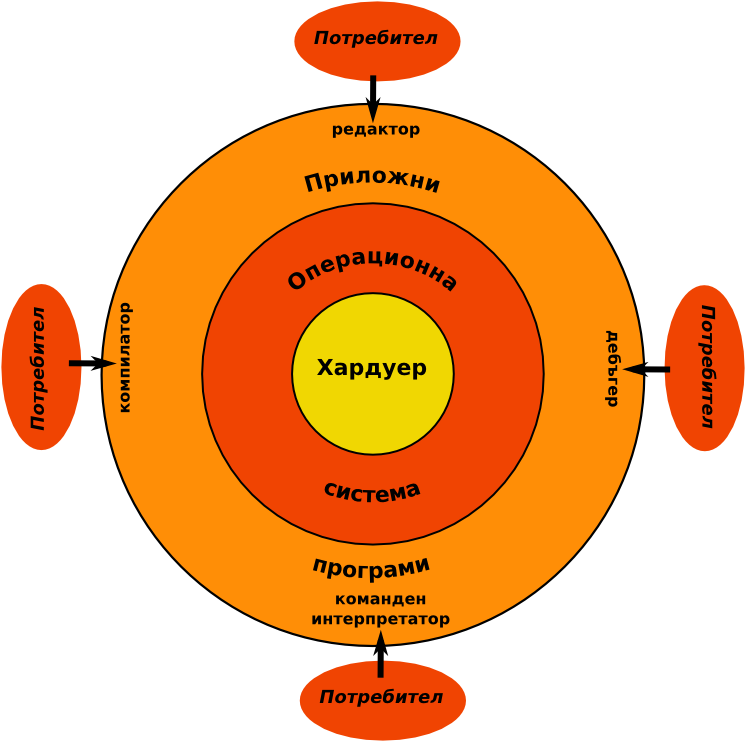
\includegraphics{pics/01-computer-structure}}
\caption{Обща структура на компютърна система}
\end{figure}
\end{frame}

%----------------------------------------------------------------- SUBSECTION -
\subsection{Задачи на операционната система}

%---------------------------------------------------------------------- SLIDE -
\begin{frame}
\frametitle{Задачи на операционната система}
\begin{itemize}
  \item Предоставя абстрактен програмен интерфейс  за работа с хардуера.
  \item Ефективно използване на компютърната система.
  \item Удобство на работа с компютъра.
  \item Способност да се развива.
\end{itemize}

\end{frame}

%----------------------------------------------------------------- SUBSECTION -
\subsection{Услуги, предоставяни от операционната система}

%---------------------------------------------------------------------- SLIDE -
\begin{frame}
\frametitle{Услуги, предоставяни от операционната система}
\begin{itemize}
  \item Разработване на програми -- редактори, компилатори, дебъгери.
  \item Изпълнение на програми.
  \item Достъп до входно/изходните устройства.
  \item Контролиран достъп до файловете.
  \item Обработка на грешки.
\end{itemize}

\end{frame}

%-------------------------------------------------------------------- SECTION -
\section{История на компютърните системи}

%----------------------------------------------------------------- SUBSECTION -
\subsection{Механични компютри}

%---------------------------------------------------------------------- SLIDE -
\begin{frame}
\frametitle{Механични компютри}
\begin{itemize}
  \item Първият цифров компютър е проектиран от 
 	\href{http://en.wikipedia.org/wiki/Charles_Babbage}{Чарлз Бабидж} (Charles
	Babbage, 1792--1871). 
\item Първоначално разработва
 \href{http://en.wikipedia.org/wiki/Difference_engine}{``разностно устройство''}, което може да се
разглежда като механичен калкулатор.
\item Проектира и се опитва да построи 
\href{http://cse.stanford.edu/classes/sophomore-college/projects-98/babbage/ana-mech.htm}{``аналитично устройство''} 
(analytical engine).
\item За 
\href{http://cse.stanford.edu/classes/sophomore-college/projects-98/babbage/ana-prog.htm}{програмиране} 
на аналитичното устройство се използват 
\href{http://en.wikipedia.org/wiki/Jacquard_loom}{перфокартите},
разработени от Жозеф Жакард.
\item Наема първият програмист -- 
\href{http://en.wikipedia.org/wiki/Ada_Lovelace}{Ада Ловелейс (Ada Lovelace)}.
\end{itemize}
\end{frame}

%---------------------------------------------------------------------- SLIDE -
\begin{frame}
\frametitle{Механични компютри}
\begin{figure}[h]
\center
\scalebox{0.3}{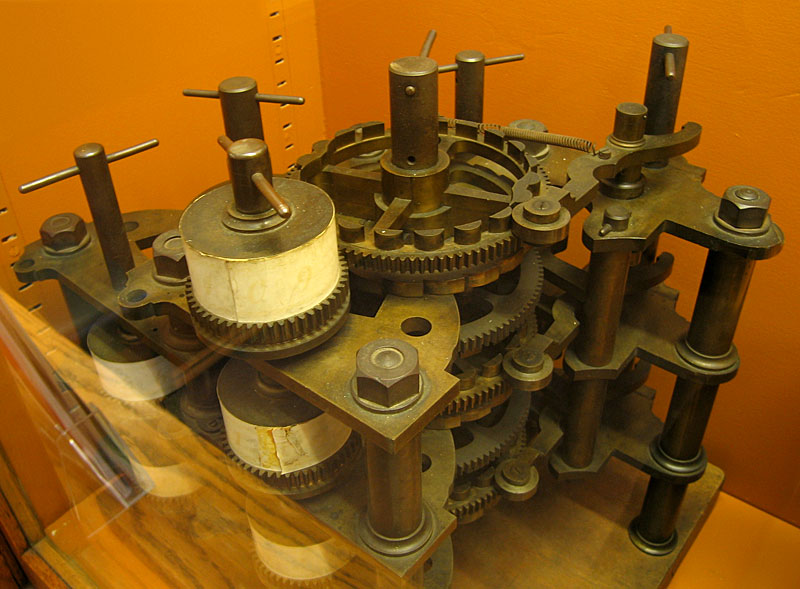
\includegraphics{pics/BabbageDifferenceEngine}}
\caption{\href{http://en.wikipedia.org/wiki/Difference_engine}{Разностното устройство на Чарлз Бабидж}}
\end{figure}
\end{frame}

%---------------------------------------------------------------------- SLIDE -
\begin{frame}
\frametitle{Механични компютри}
\begin{figure}[h]
\center
\scalebox{1.0}{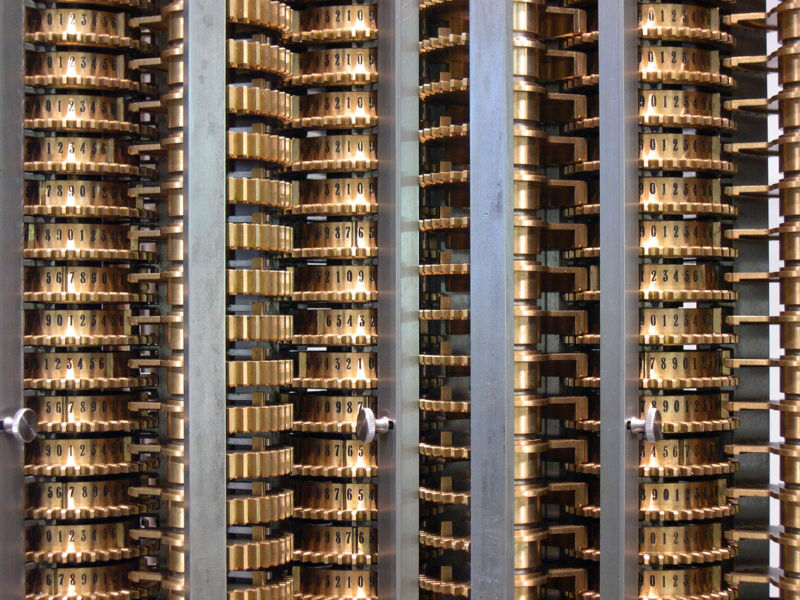
\includegraphics{pics/BabbageDifferenceEngine-800px-LondonScienceMuseumsReplicaDifferenceEngine}}
\caption{\href{http://en.wikipedia.org/wiki/Difference_engine}{Разностното устройство на Чарлз Бабидж (реплика)}}
\end{figure}
\end{frame}

%---------------------------------------------------------------------- SLIDE -
\begin{frame}
\frametitle{Механични компютри}
\begin{figure}[h]
\center
\scalebox{0.3}{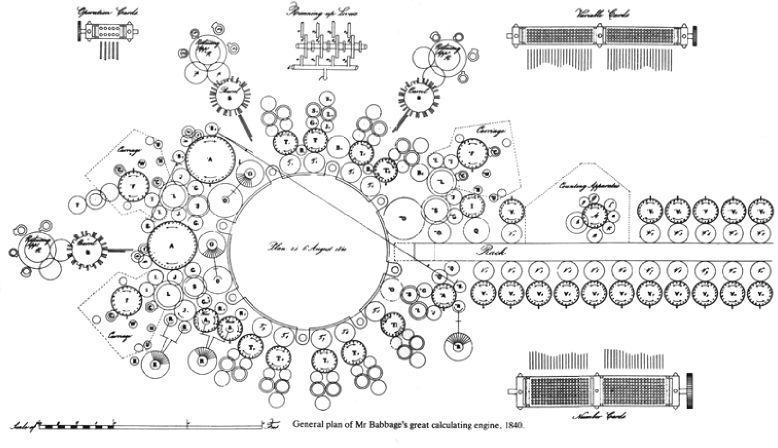
\includegraphics{pics/BabbageAnalyticalEngine-IMAGE1}}
\caption{\href{http://cse.stanford.edu/classes/sophomore-college/projects-98/babbage/ana-mech.htm}{Проект 
на аналитичното устройство на Чарлз Бабидж}}
\end{figure}
\end{frame}

%----------------------------------------------------------------- SUBSECTION -
\subsection{1940--1950}

%---------------------------------------------------------------------- SLIDE -
\begin{frame}
\frametitle{\href{http://en.wikipedia.org/wiki/History_of_computing_hardware}{1940--1950}}
\begin{itemize}
  \item Разработва се първото поколение електронни компютри.
  \item Напредък в разработването на електронни компоненти през 30-те години на
  ХХ век -- релета, вакумни лампи, кондезатори.
  \item На много места по света различни екипи успяват да конструират електронни
  цифрови изчислителни устройства.
  \item {\em ``I think there is a world market for about five computers''} --
  забележка, която се приписва на
  \href{http://en.wikipedia.org/wiki/Thomas_J._Watson}{Томас Уотсън (Thomas J. Watson)}, 
  председател на борда на директорите на IBM, 1943.  
\end{itemize}
\end{frame}

%---------------------------------------------------------------------- SLIDE -
\begin{frame}
\frametitle{\href{http://en.wikipedia.org/wiki/History_of_computing_hardware}{1940--1950}}
\begin{itemize}
  \item Като елементна база се използват релета и вакумни лампи.
  \item Възможностите на различните устройства устойчиво нарастват.
\end{itemize}
\begin{figure}[h]
\center
\scalebox{0.2}{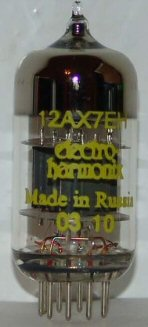
\includegraphics{pics/vacuum-tubes-Minaturevacuumtube}}\scalebox{0.30}{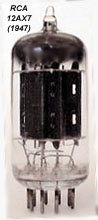
\includegraphics{pics/vacuum-tubes-RCA12ax7}}
\caption{\href{http://en.wikipedia.org/wiki/Vacuum_tube}{Вакумни лампи}}
\end{figure}

\end{frame}

%-------------------------------------------------------------- SUBSUBSECTION -
\subsubsection{Конрад Зусе -- Z3}

%---------------------------------------------------------------------- SLIDE -
\begin{frame}
\frametitle{1940--1950: 
\href{http://en.wikipedia.org/wiki/Konrad_Zuse}{Конрад Зусе} -- 
\href{http://irb.cs.tu-berlin.de/~zuse/Konrad_Zuse/en/Rechner_Z3.html}{Z3 (1938--1941)}}
\begin{figure}[h]
\center
\scalebox{0.5}{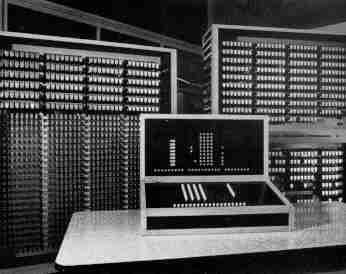
\includegraphics{pics/Z3-Rechner_Z3_1}}
\caption{\href{http://en.wikipedia.org/wiki/Z3}{Z3}}
\end{figure}
\end{frame}

%---------------------------------------------------------------------- SLIDE -
\begin{frame}
\frametitle{1940--1950: 
\href{http://en.wikipedia.org/wiki/Konrad_Zuse}{Конрад Зусе} -- 
\href{http://irb.cs.tu-berlin.de/~zuse/Konrad_Zuse/en/Rechner_Z3.html}{Z3 (1938--1941)}}
\begin{figure}[h]
\center
\scalebox{0.8}{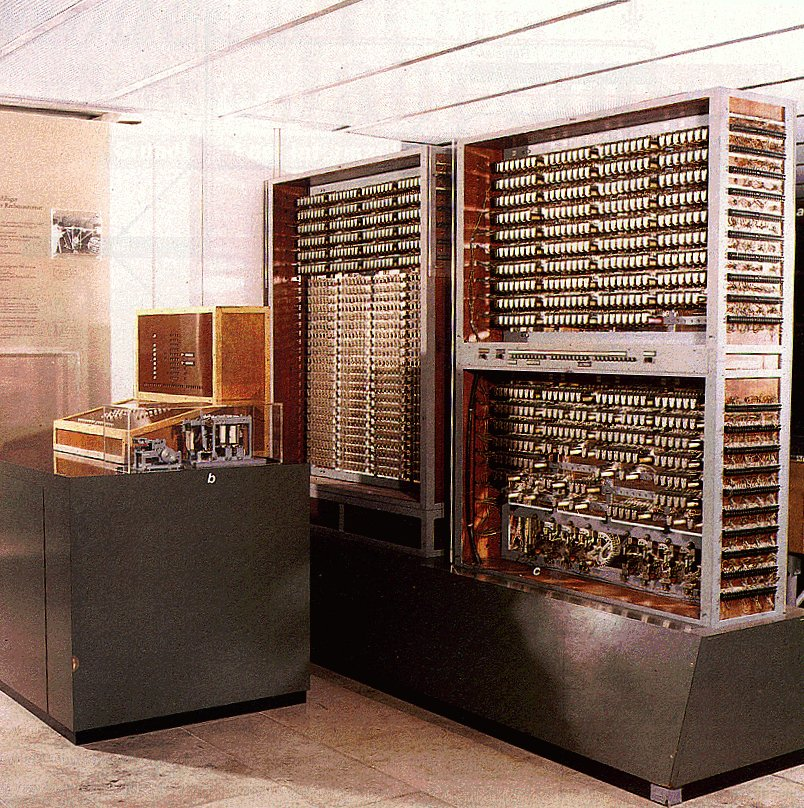
\includegraphics{pics/Z3-z3-dm}}
\caption{\href{http://en.wikipedia.org/wiki/Z3}{Z3}}
\end{figure}
\end{frame}

%-------------------------------------------------------------- SUBSUBSECTION -
\subsubsection{Компютърът на Атанасов-Бери (ABC)}

%---------------------------------------------------------------------- SLIDE -
\begin{frame}
\frametitle{1940--1950:
\href{http://en.wikipedia.org/wiki/Atanasoff-Berry_Computer}{ABC (1941)}} 
\begin{figure}[h]
\center
\scalebox{0.14}{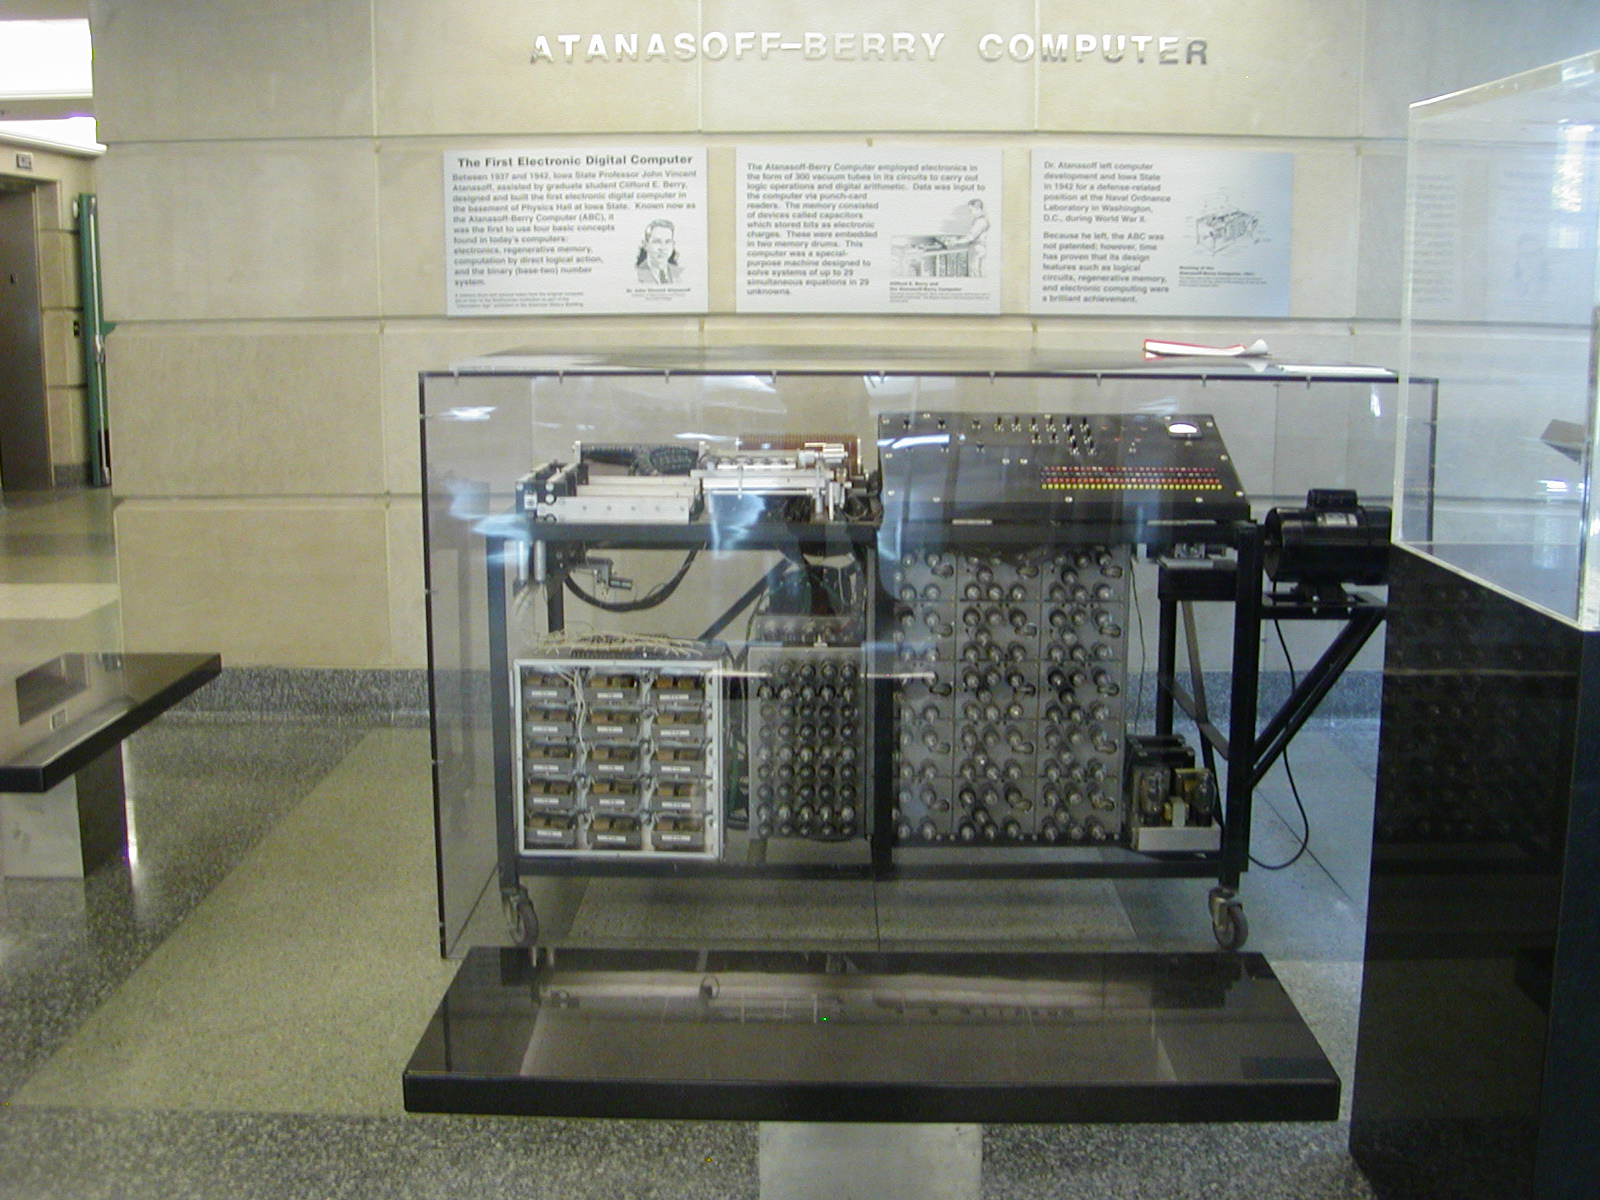
\includegraphics{pics/Atanasoff-Berry_Computer_at_Durhum_Center}}
\caption{\href{http://en.wikipedia.org/wiki/Atanasoff-Berry_Computer}{ABC
--- Компютърът на Атанасов-Бери (реплика)}}
\end{figure}
\end{frame}

%---------------------------------------------------------------------- SLIDE -
\begin{frame}
\frametitle{1940--1950: 
\href{http://en.wikipedia.org/wiki/Atanasoff-Berry_Computer}{ABC (1941)}} 
\begin{figure}[h]
\center
\scalebox{0.3}{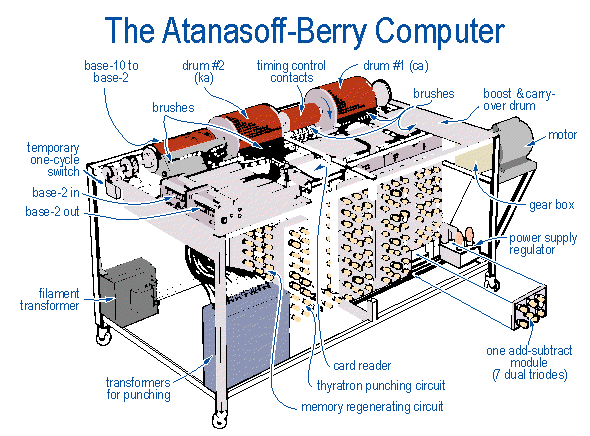
\includegraphics{pics/AtanasoffBerry-ABC}}
\caption{\href{http://en.wikipedia.org/wiki/Atanasoff-Berry_Computer}{ABC
--- Компютърът на Атанасов-Бери}}
\end{figure}
\end{frame}



%-------------------------------------------------------------- SUBSUBSECTION -
\subsubsection{Colossus}

%---------------------------------------------------------------------- SLIDE -
\begin{frame}
\frametitle{1940--1950: 
\href{http://en.wikipedia.org/wiki/Colossus_computer}{Collosus (1943)}}
\begin{figure}[h]
\center
\scalebox{0.4}{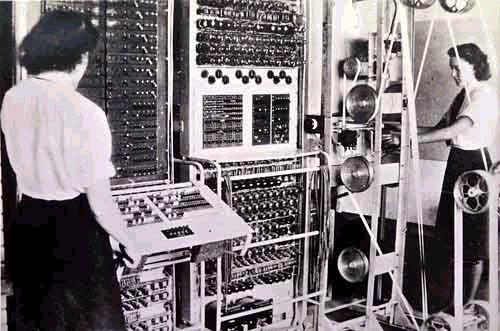
\includegraphics{pics/Colossus}}
\caption{\href{http://en.wikipedia.org/wiki/Image:Colossus.jpg}{Collosus}}
\end{figure}
\end{frame}

%---------------------------------------------------------------------- SLIDE -
\begin{frame}
\frametitle{1940--1950: 
\href{http://en.wikipedia.org/wiki/Colossus_computer}{Collosus (1943)}}
\begin{figure}[h]
\center
\scalebox{1.0}{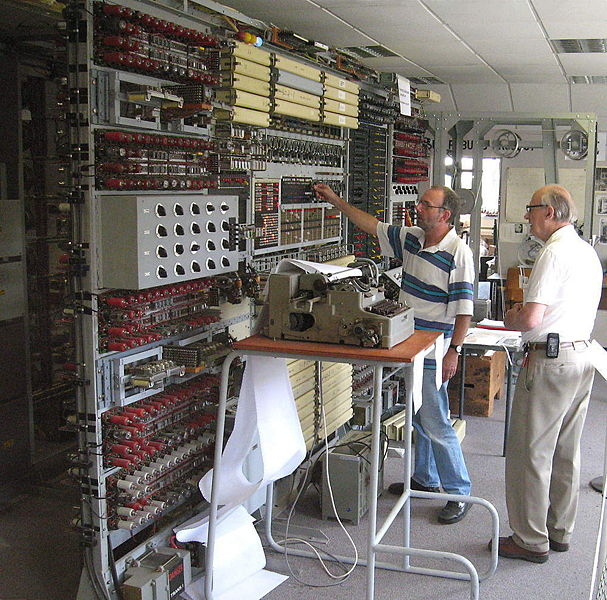
\includegraphics{pics/Colossus-320px-ColossusRebuild_11}}
\caption{\href{http://en.wikipedia.org/wiki/Image:ColossusRebuild_11.jpg}{Collosus (реплика)}}
\end{figure}
\end{frame}


%-------------------------------------------------------------- SUBSUBSECTION -
\subsubsection{Harvard Mark I – IBM ASCC}

%---------------------------------------------------------------------- SLIDE -
\begin{frame}
\frametitle{1940--1950: 
\href{http://en.wikipedia.org/wiki/Harvard_Mark_I}{Harvard Mark I – IBM ASCC (1944)}}
\begin{figure}[h]
\center
\scalebox{0.6}{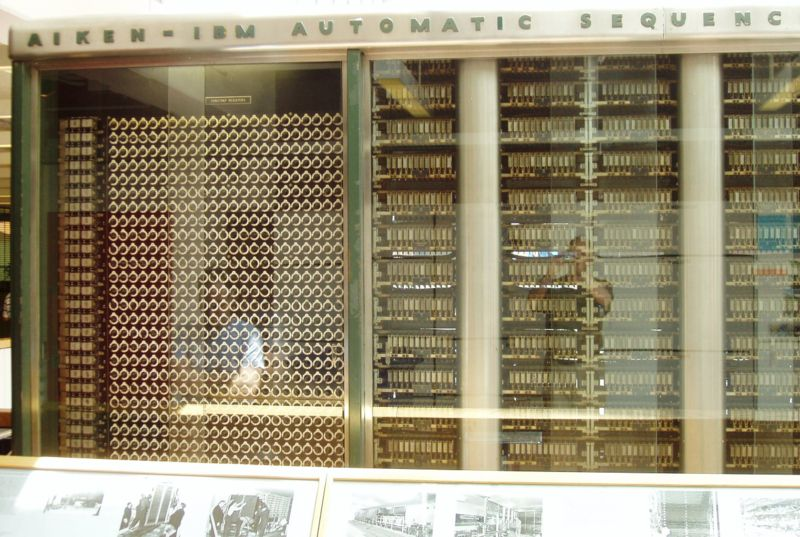
\includegraphics{pics/Harvard_Mark_I_Computer_-_Left_Segment}}
\caption{\href{http://en.wikipedia.org/wiki/Image:Harvard_Mark_I_Computer_-_Left_Segment.jpg}{Harvard Mark I
-- IBM ASCC}}
\end{figure}
\end{frame}

%---------------------------------------------------------------------- SLIDE -
\begin{frame}
\frametitle{1940--1950: 
\href{http://en.wikipedia.org/wiki/Harvard_Mark_I}{Harvard Mark I – IBM ASCC (1944)}}
\begin{figure}[h]
\center
\scalebox{0.6}{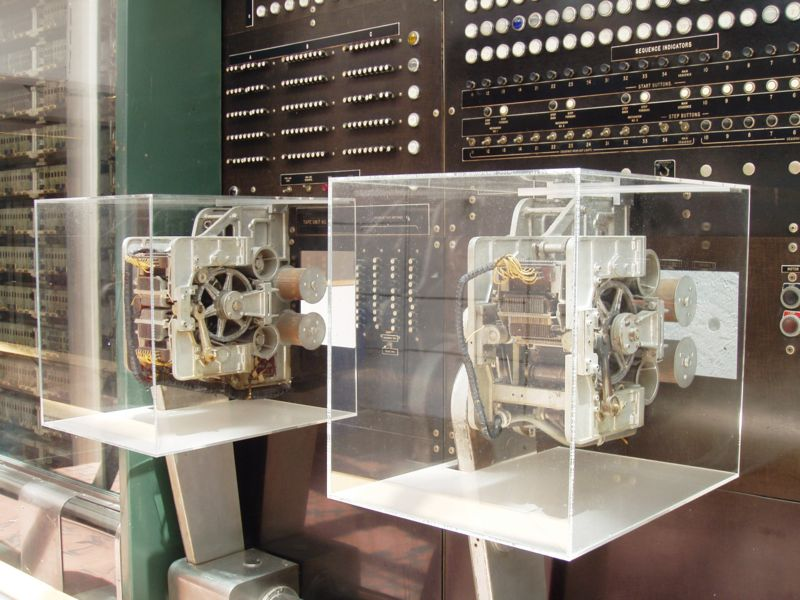
\includegraphics{pics/Harvard_Mark_I_Computer_-_Input-Output_Details}}
\caption{\href{http://en.wikipedia.org/wiki/Image:Harvard_Mark_I_Computer_-_Input-Output_Details.jpg}{Harvard Mark I
-- IBM ASCC}}
\end{figure}
\end{frame}

%---------------------------------------------------------------------- SLIDE -
\begin{frame}
\frametitle{1940--1950: 
\href{http://en.wikipedia.org/wiki/Harvard_Mark_I}{Harvard Mark I – IBM ASCC (1944)}}
\begin{figure}[h]
\center
\scalebox{0.6}{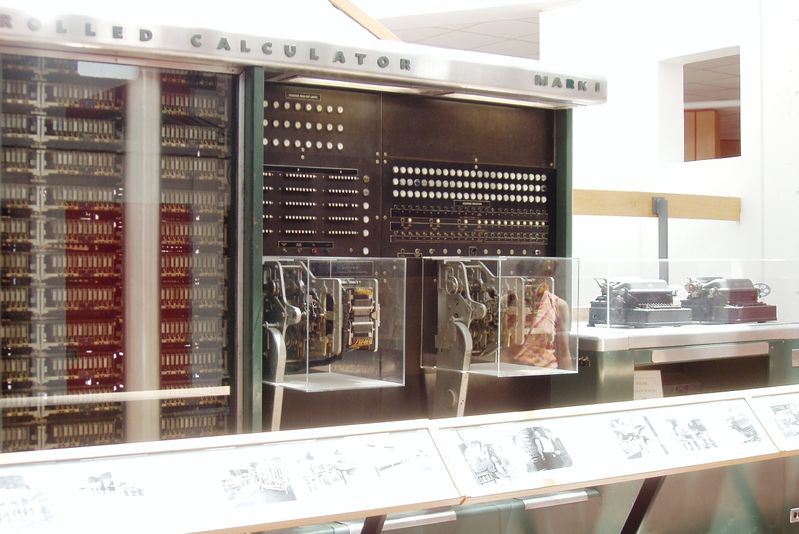
\includegraphics{pics/Harvard_Mark_I_Computer_-_Right_Segment}}
\caption{\href{http://en.wikipedia.org/wiki/Image:Harvard_Mark_I_Computer_-_Right_Segment.JPG}{Harvard Mark I
-- IBM ASCC}}
\end{figure}
\end{frame}


%-------------------------------------------------------------- SUBSUBSECTION -
\subsubsection{ENIAC}

%---------------------------------------------------------------------- SLIDE -
\begin{frame}
\frametitle{1940--1950: 
\href{http://en.wikipedia.org/wiki/ENIAC}{ENIAC (1944)}}
\begin{itemize}
  \item ENIAC -- Electronic Numerical Integrator And Computer
  \item Изграден е от 17466 вакумни лампи, 7200 диода, 1500 релета, 70000
  резистори, 10000 кондензатори, и съдържа около 7 милиона спойки.
  \item Тежи около 27 тона, заема около 170 квадратни метра.
  \item Консумира около 170 kW.
\end{itemize}
\end{frame}

%---------------------------------------------------------------------- SLIDE -
\begin{frame}
\frametitle{1940--1950: 
\href{http://en.wikipedia.org/wiki/ENIAC}{ENIAC (1944)}}
\begin{figure}[h]
\center
\scalebox{0.3}{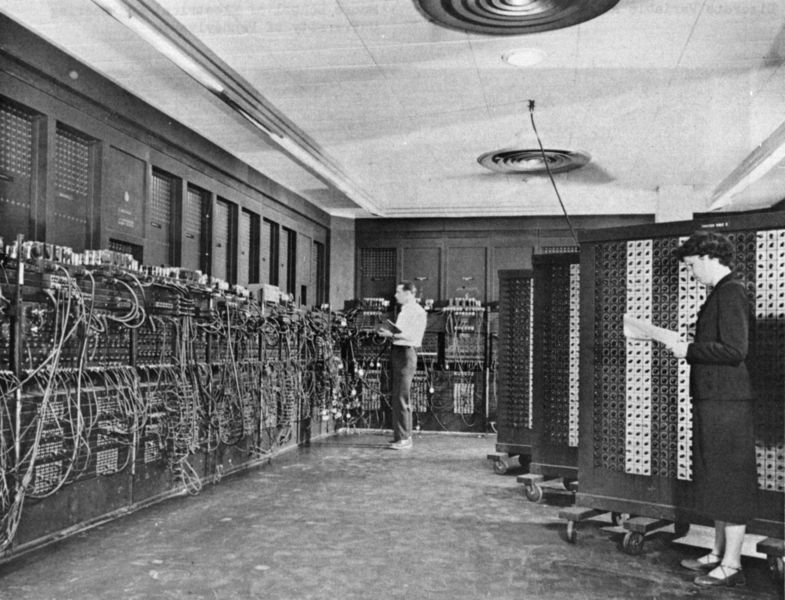
\includegraphics{pics/ENIAC-785px-Eniac}}
\caption{\href{http://en.wikipedia.org/wiki/Image:Eniac.jpg}{ENIAC}}
\end{figure}
\end{frame}

%---------------------------------------------------------------------- SLIDE -
\begin{frame}
\frametitle{1940--1950: 
\href{http://en.wikipedia.org/wiki/ENIAC}{ENIAC (1944)}}
\begin{figure}[h]
\center
\scalebox{0.4}{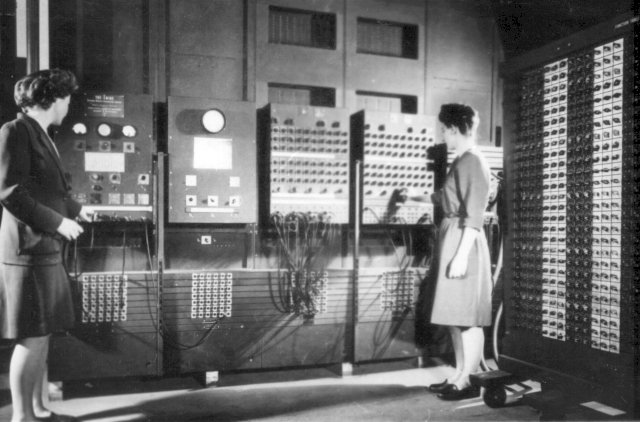
\includegraphics{pics/ENIAC-Two_women_operating_ENIAC}}
\caption{\href{http://en.wikipedia.org/wiki/Image:Two_women_operating_ENIAC.gif}{ENIAC}}
\end{figure}
\end{frame}

%---------------------------------------------------------------------- SLIDE -
\begin{frame}
\frametitle{1940--1950: 
\href{http://en.wikipedia.org/wiki/ENIAC}{ENIAC (1944)}}
\begin{figure}[h]
\center
\scalebox{0.35}{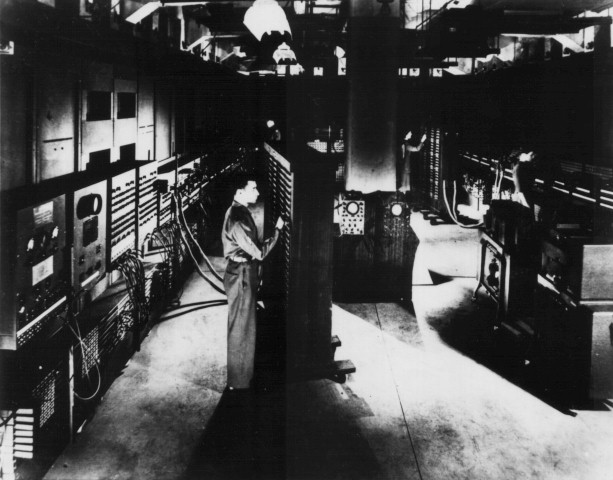
\includegraphics{pics/ENIAC-Classic_shot_of_the_ENIAC}}
\caption{\href{http://en.wikipedia.org/wiki/Image:Classic_shot_of_the_ENIAC.jpg}{ENIAC}}
\end{figure}
\end{frame}

%-------------------------------------------------------------- SUBSUBSECTION -
\subsubsection{Първо поколение компютри}

%---------------------------------------------------------------------- SLIDE -
\begin{frame}
\frametitle{1940--1950: Сравнение между първите компютри}
\begin{center}
\vfill
\begin{table}
\begin{supertabular}{|l|l|l|l|l|l|}
Компютър  & Година & \hfill\begin{rotate}{90}Бинарен\end{rotate}\hfil&
\hfill\begin{rotate}{90}Електронен\end{rotate} &
\hfill\begin{rotate}{90}Програмируем\end{rotate} &
\hfill\begin{rotate}{90}Пълен по Тюринг\end{rotate}\\
\hline
Z3 & 1941 & Да & Не & Да & Да \\
ABC & 1941 & Да & Да & Не & Не \\
Colossus & 1943 & Да & Да & Частично & Не \\
Harvard Mark I -- IBM ASCC & 1944 & Не & Не & Да & Да \\
ENIAC & 1944 & Не & Да & Частично & Да \\
\hline
\end{supertabular}
\caption{\href{http://en.wikipedia.org/wiki/Z3\#How_the_Z3_relates_to_other_work}{Сравнение 
между възможностите на ранните компютри}}

\end{table}
\end{center}
\end{frame}

%---------------------------------------------------------------------- SLIDE -
\begin{frame}
\frametitle{1940--1950: Работа и използване на компютрите}
\begin{itemize}
  \item Няма операционна система.
  \item Един екип от хора проектира, конструира, програмира, обслужва и
  поддържа всяка машина. 
  \item Компютрите са уникални (единствени) екземпляри.
  \item Програмите се пишат на машинен език. 
  \item Често за програмиране се използват и ``plugboard'' за промяна на
  опроводяването. 
\end{itemize}
\end{frame}

%---------------------------------------------------------------------- SLIDE -
\begin{frame}
\frametitle{1940--1950}
\begin{figure}[h]
\center
\scalebox{1}{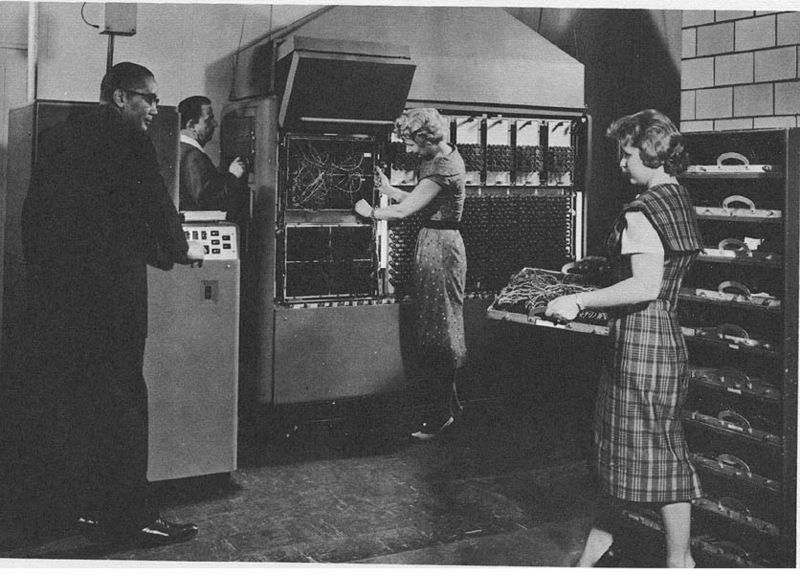
\includegraphics{pics/PLUGBOARD-800px-BRL61-UNIVAC-120}}
\caption{\href{http://en.wikipedia.org/wiki/Plug-board}{UNIVAC Plugboard}}
\end{figure}
\end{frame}

%---------------------------------------------------------------------- SLIDE -
\begin{frame}
\frametitle{1940--1950}
\begin{figure}[h]
\center
\scalebox{0.7}{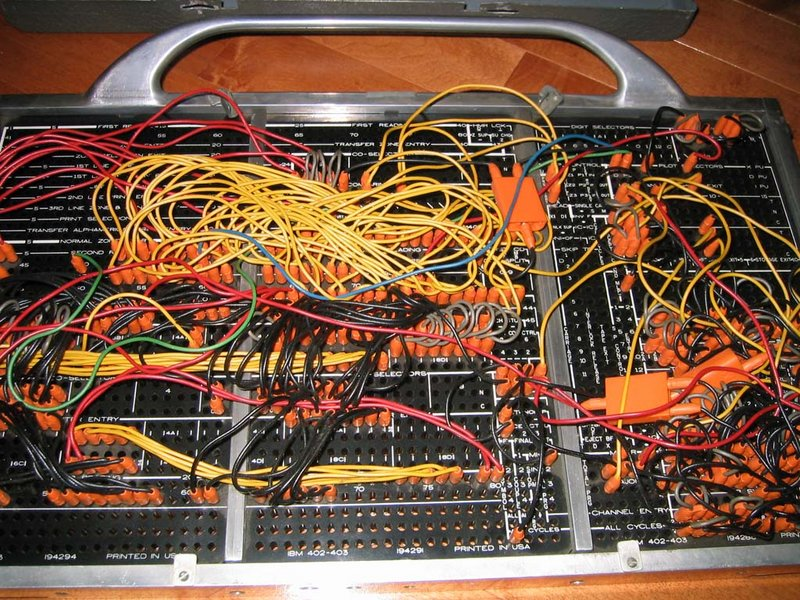
\includegraphics{pics/PLUGBOARD-800px-IBM402}}
\caption{\href{http://en.wikipedia.org/wiki/Plug-board}{IBM 402 Plugboard}}
\end{figure}
\end{frame}


%----------------------------------------------------------------- SUBSECTION -
\subsection{1950--1960}

%---------------------------------------------------------------------- SLIDE -
\begin{frame}
\frametitle{\href{http://en.wikipedia.org/wiki/History_of_computing_hardware}{1950--1960}}
\begin{itemize}
  \item Компютрите стават достатъчно надеждни и вече могат да се произвеждат и
  продават на потребителите.
  \item Появява се разделение между разработчиците на компютри, производители,
  оператори, програмисти и поддържащ персонал.
  \item Започват да включват програмно осигуряване, което улеснява преминаването
  от едно задание към друго.
  \item В елементната база на компютрите започват да навлиза транзисторът.
\end{itemize}
\begin{figure}[h]
\center
\scalebox{0.2}{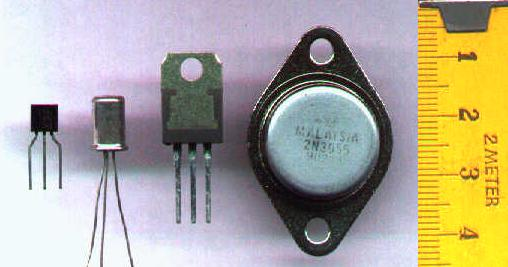
\includegraphics{pics/Transistor-photo}}
\caption{\href{http://en.wikipedia.org/wiki/Transistor}{Транзистори}}
\end{figure}
\end{frame}

%-------------------------------------------------------------- SUBSUBSECTION -
\subsubsection{UNIVAC I}


%---------------------------------------------------------------------- SLIDE -
\begin{frame}
\frametitle{1950--1960: \href{http://en.wikipedia.org/wiki/UNIVAC_I}{UNIVAC I}}
\begin{itemize}
  \item През 1951 е доставен първият комерсиален масово произвеждан компютър --
  UNIVAC I.
  \item Произвежда се от компанията Remington Rand.
  \item Произведени са около 46 компютъра.
  \item Във всеки компютър се използват около 7200 вакумни лампи.
  \item Консумацията на електроенергия е около 125kW.
  \item Оперативната памет се състои от 1000 думи, като всяка дума е 72 битова --
  т.е. около 9k.
\end{itemize}
\end{frame}

%---------------------------------------------------------------------- SLIDE -
\begin{frame}
\frametitle{1950--1960: \href{http://en.wikipedia.org/wiki/UNIVAC_I}{UNIVAC I}}
\begin{figure}[h]
\center
\scalebox{1.0}{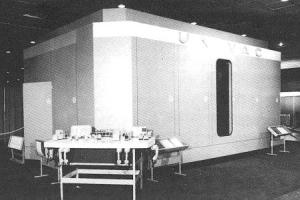
\includegraphics{pics/UNIVAC-I}}
\caption{\href{http://en.wikipedia.org/wiki/Image:UNIVAC-I.JPG}{UNIVAC I:
Централен процесор}}
\end{figure}
\end{frame}

%---------------------------------------------------------------------- SLIDE -
\begin{frame}
\frametitle{1950--1960: \href{http://en.wikipedia.org/wiki/UNIVAC_I}{UNIVAC I}}
\begin{figure}[h]
\center
\scalebox{0.45}{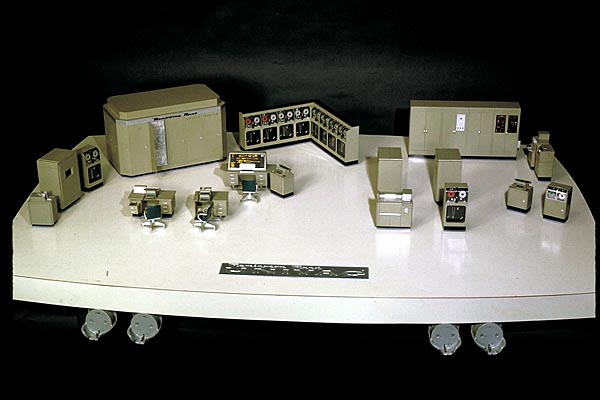
\includegraphics{pics/Univac-model}}
\caption{\href{http://americanhistory.si.edu/collections/comphist/objects/univac.htm}{UNIVAC I:
Умален модел}}
\end{figure}
\end{frame}

%-------------------------------------------------------------- SUBSUBSECTION -
\subsubsection{IBM 700}

%---------------------------------------------------------------------- SLIDE -
\begin{frame}
\frametitle{1950--1960: \href{http://en.wikipedia.org/wiki/IBM_700/7000_series}{IBM 700}}
\begin{itemize}
  \item През 1952 IBM обявява първият си електронен компютър IBM 701.
  \item 
  \href{http://www-03.ibm.com/ibm/history/exhibits/701/701_1415bx01.html}{IBM
  701} е първият от серията големи машини (mainframe) на IBM 700/7000.  
  \item \href{http://en.wikipedia.org/wiki/IBM_704}{IBM 704} се появява през
  1954 и е пъвият компютър който използва магнитна памет (core memory).
\end{itemize}
\end{frame}
        
%---------------------------------------------------------------------- SLIDE -
\begin{frame}
\frametitle{1950--1960: \href{http://en.wikipedia.org/wiki/IBM_701}{IBM 701}}
\begin{figure}[h]
\center
\scalebox{0.45}{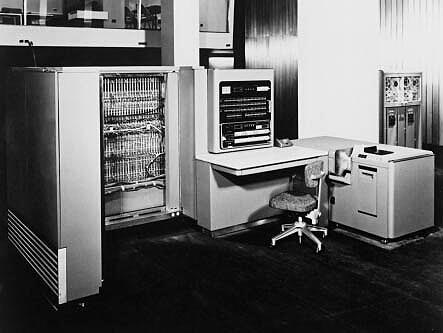
\includegraphics{pics/IBM701-141511}}
\caption{\href{http://www-03.ibm.com/ibm/history/exhibits/701/701_1415bx01.html}{IBM
701}}
\end{figure}
    
\end{frame}
   
%---------------------------------------------------------------------- SLIDE -
\begin{frame}
\frametitle{1950--1960: \href{http://en.wikipedia.org/wiki/IBM_704}{IBM 704}}
\begin{figure}[h]
\center
\scalebox{0.6}{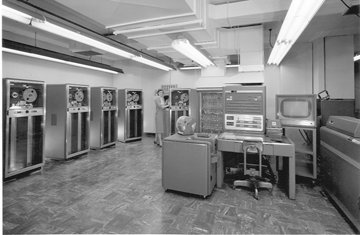
\includegraphics{pics/Ibm704}}
\caption{\href{http://en.wikipedia.org/wiki/Image:Ibm704.gif}{IBM
704}}
\end{figure}
    
\end{frame}

%-------------------------------------------------------------- SUBSUBSECTION -
\subsubsection{Fortran}

%---------------------------------------------------------------------- SLIDE -
\begin{frame}
\frametitle{1950--1960: \href{http://en.wikipedia.org/wiki/IBM_701}{IBM 704: Fortran}}
\begin{itemize}
\item През 1955-1957 е разработен и първият език за програмиране от високо ниво
\href{http://en.wikipedia.org/wiki/Fortran}{Fortran} е разработен за IBM 704.
\item През 1953 Джон Бакус прави предложение за разработване на алтернатива на
асемблер. 
\item В средата на 1954 е завършена спецификацията на FORTRAN.  
\item Ръководство за работа са FORTRAN се появява през октомври 1956.
\item Компилаторът започва да се разпространява през април 1957.
\end{itemize}
\end{frame}

%-------------------------------------------------------------- SUBSUBSECTION -
\subsubsection{Твърди дискове}

%---------------------------------------------------------------------- SLIDE -
\begin{frame}
\frametitle{1950--1960: \href{http://en.wikipedia.org/wiki/IBM_305_RAMAC}{IBM 305 RAMAC}}
\begin{itemize}
\item През 1956 IBM започва да доставя първият компютър, използващ твърди
дискове -- IBM 305.
\end{itemize}
\begin{figure}[h]
\center
%\scalebox{0.3}{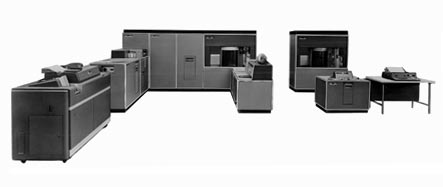
\includegraphics{pics/IBM305-PH0305}}%
\hfill\scalebox{0.35}{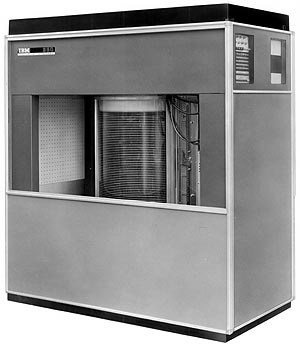
\includegraphics{pics/IBM350-PH0350A}}%
\hfill\scalebox{0.45}{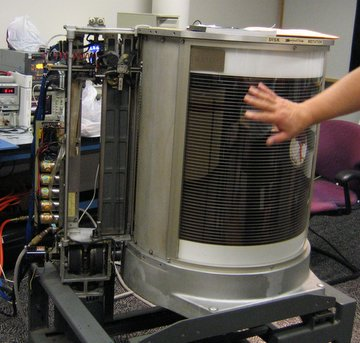
\includegraphics{pics/IBM-350-Ramac}}\hfill
\caption{\href{http://en.wikipedia.org/wiki/Early_IBM_disk_storage\#IBM_350}{IBM 350}}
\end{figure}
\end{frame}

%-------------------------------------------------------------- SUBSUBSECTION -
\subsubsection{IBM 7000}

%---------------------------------------------------------------------- SLIDE -
\begin{frame}
\frametitle{1950--1960: \href{http://en.wikipedia.org/wiki/IBM_7090}{IBM 7090}}
\begin{itemize}
  \item В края на 50-те години IBM правят подобрения на серията компютри IBM 700.
  \item Елементната база преминава към транзистори.
  \item През ноември 1959 за първи път е инсталиран IBM 7090.
  \item IBM 7090 използва думи с дължина 36 бита. Оперативната му памет е с
  размер около 32k.
  \item Типична цена на системата през 1960 е около \$2,900,000.
\end{itemize}
\end{frame}

%---------------------------------------------------------------------- SLIDE -
\begin{frame}
\frametitle{1950--1960: \href{http://en.wikipedia.org/wiki/IBM_7090}{IBM 7090}}
\begin{figure}[h]
\center
\scalebox{0.35}{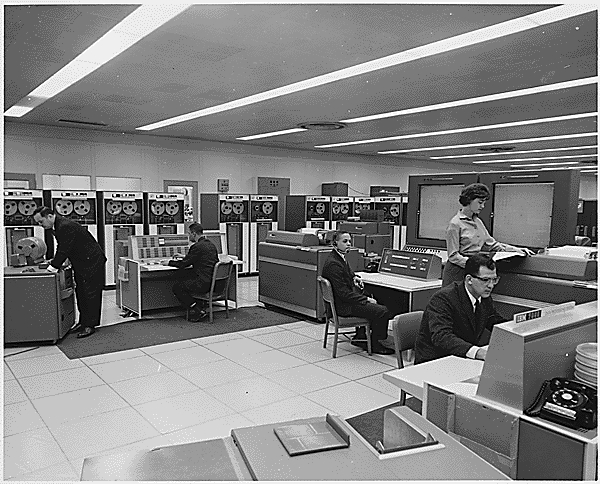
\includegraphics{pics/IBM7090-NASAComputerRoom7090}}
\caption{\href{http://en.wikipedia.org/wiki/Image:NASAComputerRoom7090.NARA.jpg}{IBM 7090}}
\end{figure}
\end{frame}

% %---------------------------------------------------------------------- SLIDE -
% \begin{frame}
% \frametitle{1950--1960: \href{http://en.wikipedia.org/wiki/IBM_7090}{IBM 7090}}
% \begin{figure}[h]
% \center
% \scalebox{0.7}{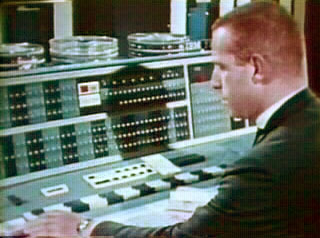
\includegraphics{pics/IBM_7090_console}}
% \caption{\href{http://en.wikipedia.org/wiki/Image:IBM_7090_console.nasa.jpg}{IBM 7090}}
% \end{figure}
% \end{frame}

%---------------------------------------------------------------------- SLIDE -
\begin{frame}
\frametitle{1950--1960: \href{http://en.wikipedia.org/wiki/IBM_7090}{IBM 7090}}
\begin{figure}[h]
\center
\scalebox{0.6}{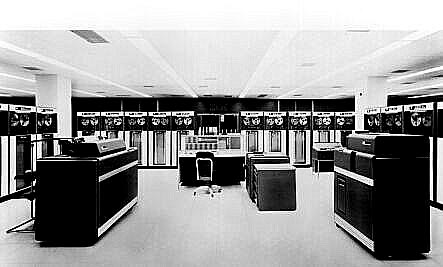
\includegraphics{pics/IBM7090-2423PH7090}}
\caption{\href{http://www-03.ibm.com/ibm/history/exhibits/mainframe/mainframe_PP7090.html}{IBM 7090}}
\end{figure}
\end{frame}


%-------------------------------------------------------------- SUBSUBSECTION -
\subsubsection{Пакетна обработка}

%---------------------------------------------------------------------- SLIDE -
\begin{frame}
\frametitle{1950--1960: Пакетна обработка}
\begin{itemize}
  \item Заданията се групират в пакети за последователно
  изпълнение.
  \item Системна програма {\em монитор}, която контролира изпълнението на
  заданията. 
  \item Част от монитора винаги се намира в паметта -- резидентен монитор.
  \item При стартиране на системата се зарежда монитора и управлението се
  предава на него.
  \item Работа на монитора е да зареди следващото задание и да предаде
  управлението на него.
  \item Когато дадена програма завърши своето изпълнение управлението се предава
  обратно на монитора.
\end{itemize}
\end{frame}

%---------------------------------------------------------------------- SLIDE -
\begin{frame}
\frametitle{1950--1960: Пакетна обработка}
\begin{itemize}
  \item Разработват се специализирани езици за управление на заданията (Job
  Control Language -- JCL):
  \begin{itemize}
    \item специализиран език за програмиране;
    \item дава инструкции на монитора какъв компилатор да използва, от къде да
    вземе данните за програмата и т.н.
  \end{itemize}
  \item Заедно с развитието на пакетната обработка се развива и хардуера,
  необходим за поддръжка на пакетна обработка на заданията:
  \begin{itemize}
    \item защита на паметта -- не позволява на работещите програми да променят
    областта от паметта, в която е разположен монитора;
    \item таймери -- предпазват системата от задания, които никога не свършват.
  \end{itemize}
\end{itemize}
\end{frame}


%---------------------------------------------------------------------- SLIDE -
\begin{frame}
\frametitle{1950--1960: \href{http://en.wikipedia.org/wiki/Punch_card}{Перфокарти}}
\begin{itemize}
  \item През този период основен интерфейс за въвеждане на програми и данни в
  компютрите са перфокартите.
\end{itemize}
\begin{figure}[h]
\center
\scalebox{0.38}{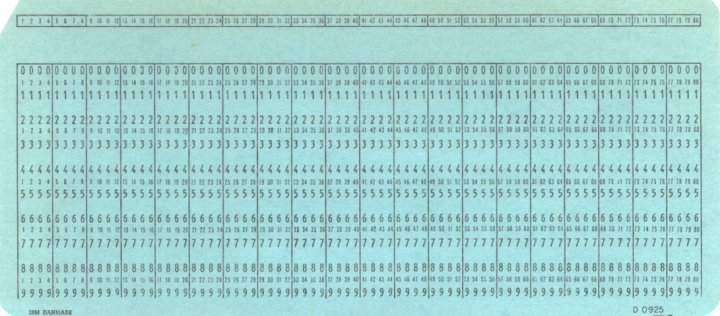
\includegraphics{pics/Punch-card-blue}}
\scalebox{0.15}{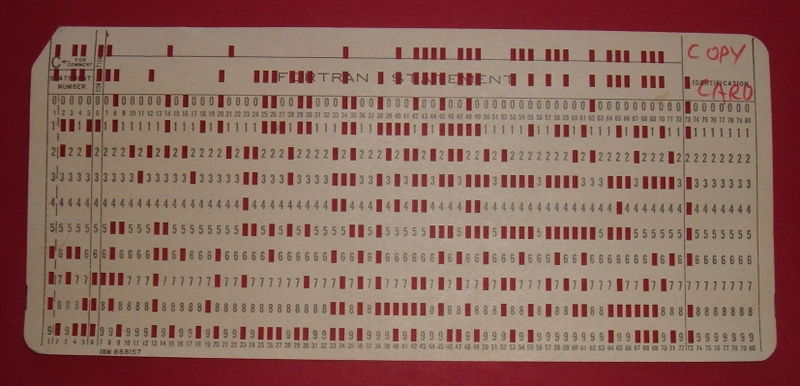
\includegraphics{pics/punch-card-800px-IBM1130CopyCard}}
\caption{\href{http://en.wikipedia.org/wiki/Punch_card}{Перфокарти}}
\end{figure}

\end{frame}


%---------------------------------------------------------------------- SLIDE -
\begin{frame}
\frametitle{1950--1960: \href{http://en.wikipedia.org/wiki/Punch_card}{Перфокарти}}
\begin{figure}[h]
\center
\scalebox{0.21}{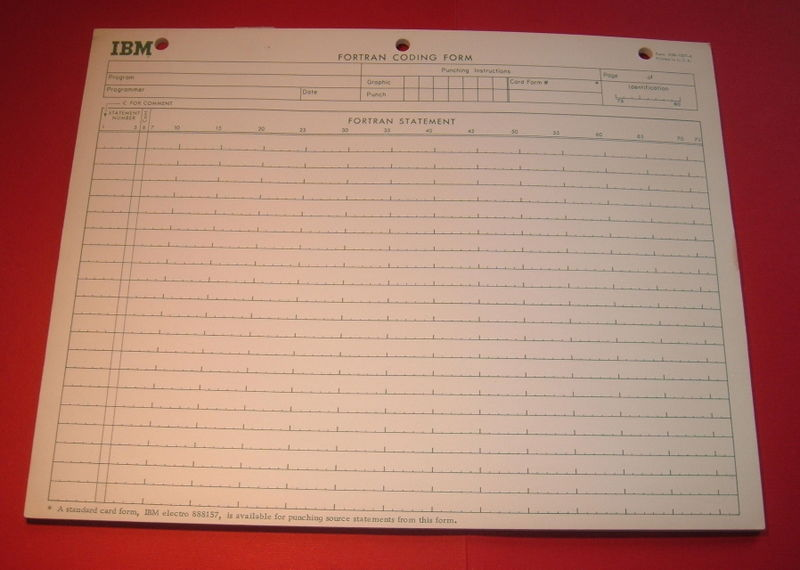
\includegraphics{pics/punch-card-800px-FortranCodingForm}}
\scalebox{0.2}{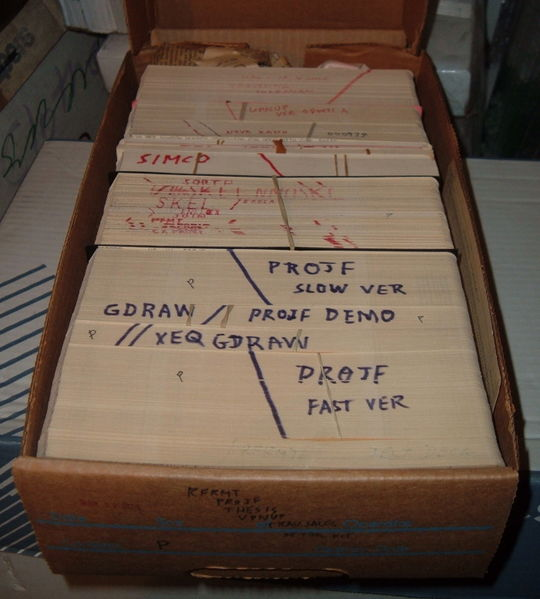
\includegraphics{pics/punch-card-540px-PunchCardDecks}}
\caption{\href{http://en.wikipedia.org/wiki/Punch_card}{Перфокарти}}
\end{figure}
\end{frame}


%----------------------------------------------------------------- SUBSECTION -
\subsection{1960--1970}

%---------------------------------------------------------------------- SLIDE -
\begin{frame}
\frametitle{\href{http://en.wikipedia.org/wiki/History_of_computing_hardware_(1960s-present)}{
1960--1970}}
\begin{itemize}
  \item В края на 50-те години са създадени първите интегрални схеми --
  микрочипове.
  \item Първите компютри, които използват микрочипове, се появяват през 1963.
  \item Цената на компютрите започва да спада, а надеждността им -- нараства.
  \item Комптютрите започват да се използват масово -- всеки университет, всяка
  по-голяма или средна компания.
  \item Операционните системи са основно за пакетна обработка.
  \item Въвеждат се многозадачността (multiprogramming) и времеделението
  (timesharing). 
\end{itemize}
\end{frame}


%-------------------------------------------------------------- SUBSUBSECTION -
\subsubsection{IBM System/360}

%---------------------------------------------------------------------- SLIDE -
\begin{frame}
\frametitle{1960--1970: \href{http://en.wikipedia.org/wiki/System/360}{IBM System/360}}
\begin{itemize}
  \item През 1964 IBM въвежда серията от компютри
  \href{http://www-03.ibm.com/ibm/history/exhibits/mainframe/mainframe_PR360.html}{System/360}. 
  \item Серията се рекламира като компютър с общо предназначение и с пълна
  функционалност. От там произлиза 360 - пълен кръг 360 градуса.
  \item Моделите варират от 360/20 до 360/65. По-късно са въведени и 360/95.
  Типичните конфигурации включват памет в диапазона от 16K до 1024K.
  \item  Цените на компютри от серията System/360 варират от около \$130,000
  до около \$5,500,000.
  \item Тъй като компютрите в серията са напълно съвместими е възможно
  потребителят да започне с "евтин компютър" от ниския ценови диапазон, и при
  нужда да надгражда системата си.
\end{itemize}
\end{frame}
  
%---------------------------------------------------------------------- SLIDE -
\begin{frame}
\frametitle{1960--1970: \href{http://en.wikipedia.org/wiki/System/360}{IBM System/360}}
\begin{itemize}
  \item Операционната система разработена от IBM за System/360 е OS/360.
  \item "The Mythical Man-Month: Essays on Software Engineering", Fred Brooks,
  Addison-Wesley, 1975, ISBN 0-201-00650-2
  \item Основното предимство на "фамилия" от съвместими компютри се превръща
  същевременно и в основна слабост.
  \item Идеята е целият софтуер (включително и операционната система) да работи
  без промени върху всички модели от фамилията. 
  \item Различните модели, обаче, се различават твърде много. В резултат се
  получава огромна и извънредно сложна операционна система.
\end{itemize}
\end{frame}
\item 
  
%---------------------------------------------------------------------- SLIDE -
\begin{frame}
\frametitle{1960--1970: \href{http://en.wikipedia.org/wiki/System/360}{IBM
System/360}} 
\begin{columns}
\column{0.7\textwidth}
\begin{itemize}
  \item Една от най-важните концепции, въведени в OS/360 е многозадачността.
  \item Друга важна концепция въведена в OS/360 е спулинга (spooling, SPOOL -
  Simultaneous Peripheral Operation On Line) 
\end{itemize}
\column{0.3\textwidth}
\begin{figure}
\center
\scalebox{0.5}{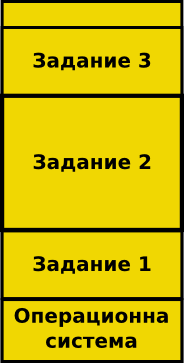
\includegraphics{pics/01-multiprogramming}}
\caption{Многозадачност}
\end{figure}
\end{columns}
\end{frame}

%---------------------------------------------------------------------- SLIDE -
\begin{frame}
\frametitle{1960--1970: \href{http://en.wikipedia.org/wiki/System/360}{IBM
System/360}} 
\begin{figure}
\center
\scalebox{1}{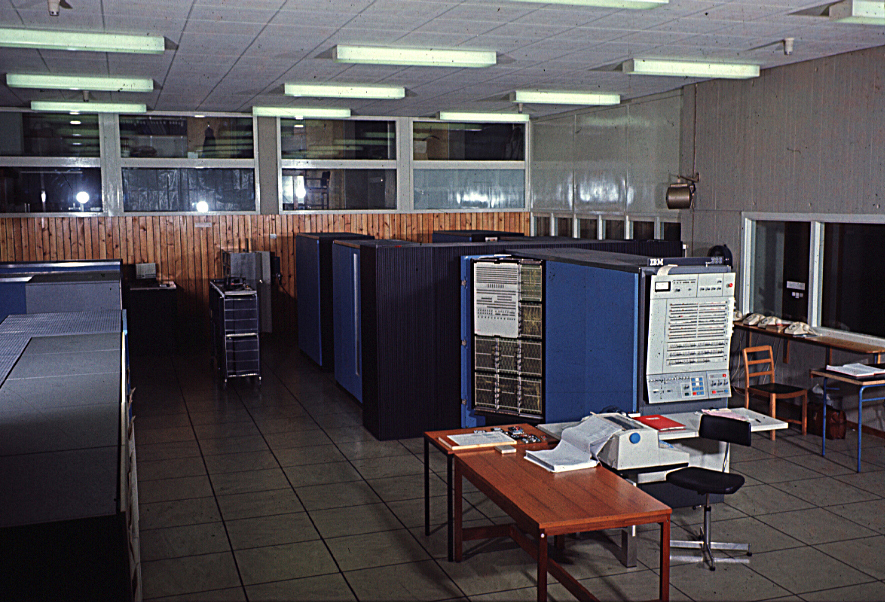
\includegraphics{pics/IBM-System-360-slide07}}
\caption{\href{http://www.cs.newcastle.ac.uk/events/anniversaries/40th/images/ibm360_672/index.html}{IBM System 360/65}}
\end{figure}
\end{frame}

%---------------------------------------------------------------------- SLIDE -
\begin{frame}
\frametitle{1960--1970: \href{http://en.wikipedia.org/wiki/System/360}{IBM
System/360}} 
\begin{figure}
\center
\scalebox{1}{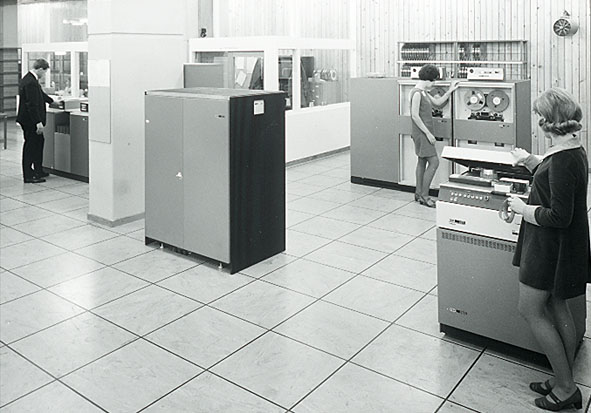
\includegraphics{pics/IBM-System-360-28}}
\caption{\href{http://www.cs.newcastle.ac.uk/events/anniversaries/40th/images/ibm360_672/index.html}{IBM System 360/65}}
\end{figure}
\end{frame}

%---------------------------------------------------------------------- SLIDE -
\begin{frame}
\frametitle{1960--1970: \href{http://en.wikipedia.org/wiki/System/360}{IBM
System/360}} 
\begin{figure}
\center
\scalebox{1}{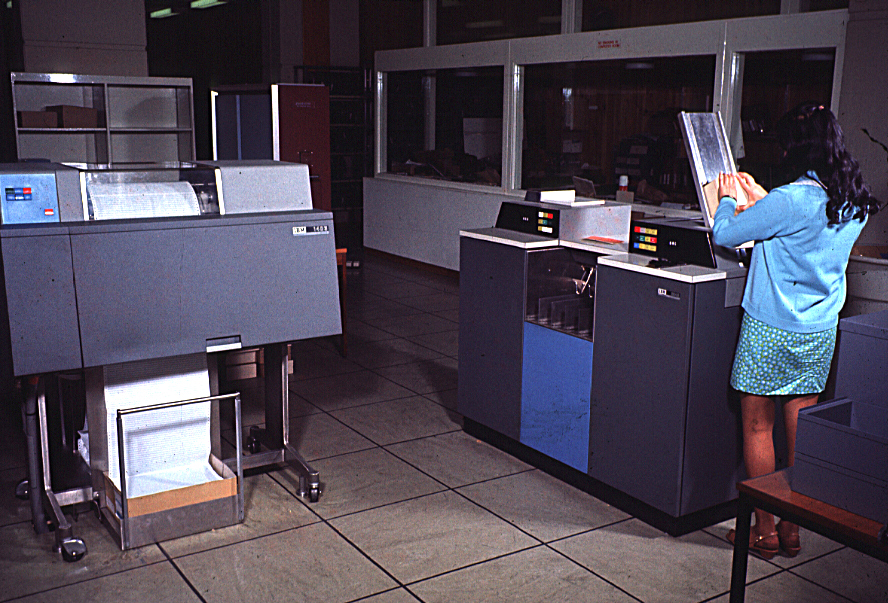
\includegraphics{pics/IBM-System-360-slide19}}
\caption{\href{http://www.cs.newcastle.ac.uk/events/anniversaries/40th/images/ibm360_672/index.html}{IBM System 360/65}}
\end{figure}
\end{frame}


%-------------------------------------------------------------- SUBSUBSECTION -
\subsubsection{Миникомпютри}

%---------------------------------------------------------------------- SLIDE -
\begin{frame}
\frametitle{1960--1970: \href{http://en.wikipedia.org/wiki/Minicomputer}{Миникомпютри}}
\begin{itemize}
  \item В началото на 60-те години стартира производството и предлагането на
  миникомпютри. 
  \item Термина {\em миникомпютър} се използва за ``малък'' компютър.
  \item Най-известния производител на миникомпютри е Digital Equipment
  Corporation (DEC).
\end{itemize}
\end{frame}

%---------------------------------------------------------------------- SLIDE -
\begin{frame}
\frametitle{1960--1970: \href{http://en.wikipedia.org/wiki/PDP-1}{PDP-1}}
\begin{itemize}
  \item Един от първите миникомпютри е
  \href{http://en.wikipedia.org/wiki/PDP-1}{PDP-1} на Digital Equipment, който
  е въведен през 1961.
  \item PDP-1 използва думи с дължина 18 бита. Стандартно оперативната му памет
  съдържа 4K думи с дължина 18 бита (това е еквивалентно на около 9KB). Паметта му
  може да се разшири до 64K думи (т.е около 144KB).
  \item Процесорът на PDP-1 е бил в състояние да извърши около 100000
  аритметични операции в секунда.
  \item Но тъй като цената му е "само"\  \$120,000 се превръща в небивал
  търговски успех.
\end{itemize}
\end{frame}

%---------------------------------------------------------------------- SLIDE -
\begin{frame}
\frametitle{1960--1970: \href{http://en.wikipedia.org/wiki/PDP-1}{PDP-1}}
\begin{figure}
\center
\scalebox{0.6}{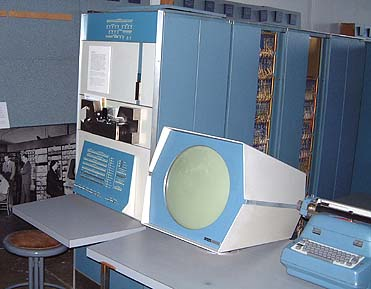
\includegraphics{pics/PDP-1-Vs-dec-pdp-1}}
\caption{\href{http://en.wikipedia.org/wiki/Image:Vs-dec-pdp-1.jpg}{PDP-1}}
\end{figure}
\end{frame}

%---------------------------------------------------------------------- SLIDE -
\begin{frame}
\frametitle{1960--1970: \href{http://en.wikipedia.org/wiki/PDP-8}{PDP-8}}
\begin{itemize}
  \item Първият истински успешен миникомпютър на Digital Equipment е PDP-8.
  \item PDP-8 е серия от съвместими 12 битови миникомпютри.
  \item Продажбите на PDP-8 започват през 1964.
  \item Базовата конфигурация включвала около
  6KB оперативна памет, разширяема до около 48KB.
  \item При излизането му на пазара цената на базовата конфугурация била ``само''
  \$16000. 
\end{itemize}
\end{frame}  

%---------------------------------------------------------------------- SLIDE -
\begin{frame}
\frametitle{1960--1970: \href{http://en.wikipedia.org/wiki/PDP-8}{PDP-8}}
\begin{figure}
\center
\scalebox{0.3}{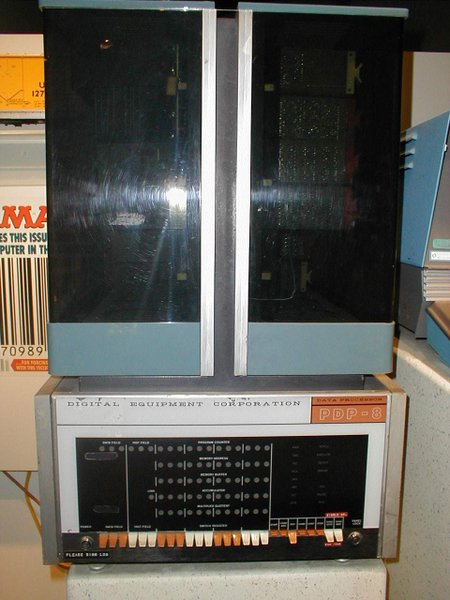
\includegraphics{pics/PDP-8-450px-PDP-8}}
\caption{\href{http://en.wikipedia.org/wiki/Image:PDP-8.jpg}{PDP-8}}
\end{figure}
\end{frame}

%---------------------------------------------------------------------- SLIDE -
\begin{frame}
\frametitle{1960--1970: \href{http://en.wikipedia.org/wiki/PDP-11}{PDP-11}}
\begin{columns}
\column{0.6\textwidth}
\begin{itemize}
  \item  Кулминация на серията миникомпютри на DEC е
  \href{http://en.wikipedia.org/wiki/PDP-11}{PDP-11}. 
  \item PDP-11 е серия от съвместими 16-битови миникомпютри.
  \item PDP-11 се появява на пазара през 70-те години.
%   \item The PDP-11 was a series of 16-bit minicomputers sold by Digital
%   Equipment Corp. in the 1970s and 1980s. The PDP-11 was a successor to DEC's
%   PDP-8 computer in the PDP series of computers.  
\end{itemize}
\column{0.4\textwidth}
\begin{figure}
\center
\scalebox{0.2}{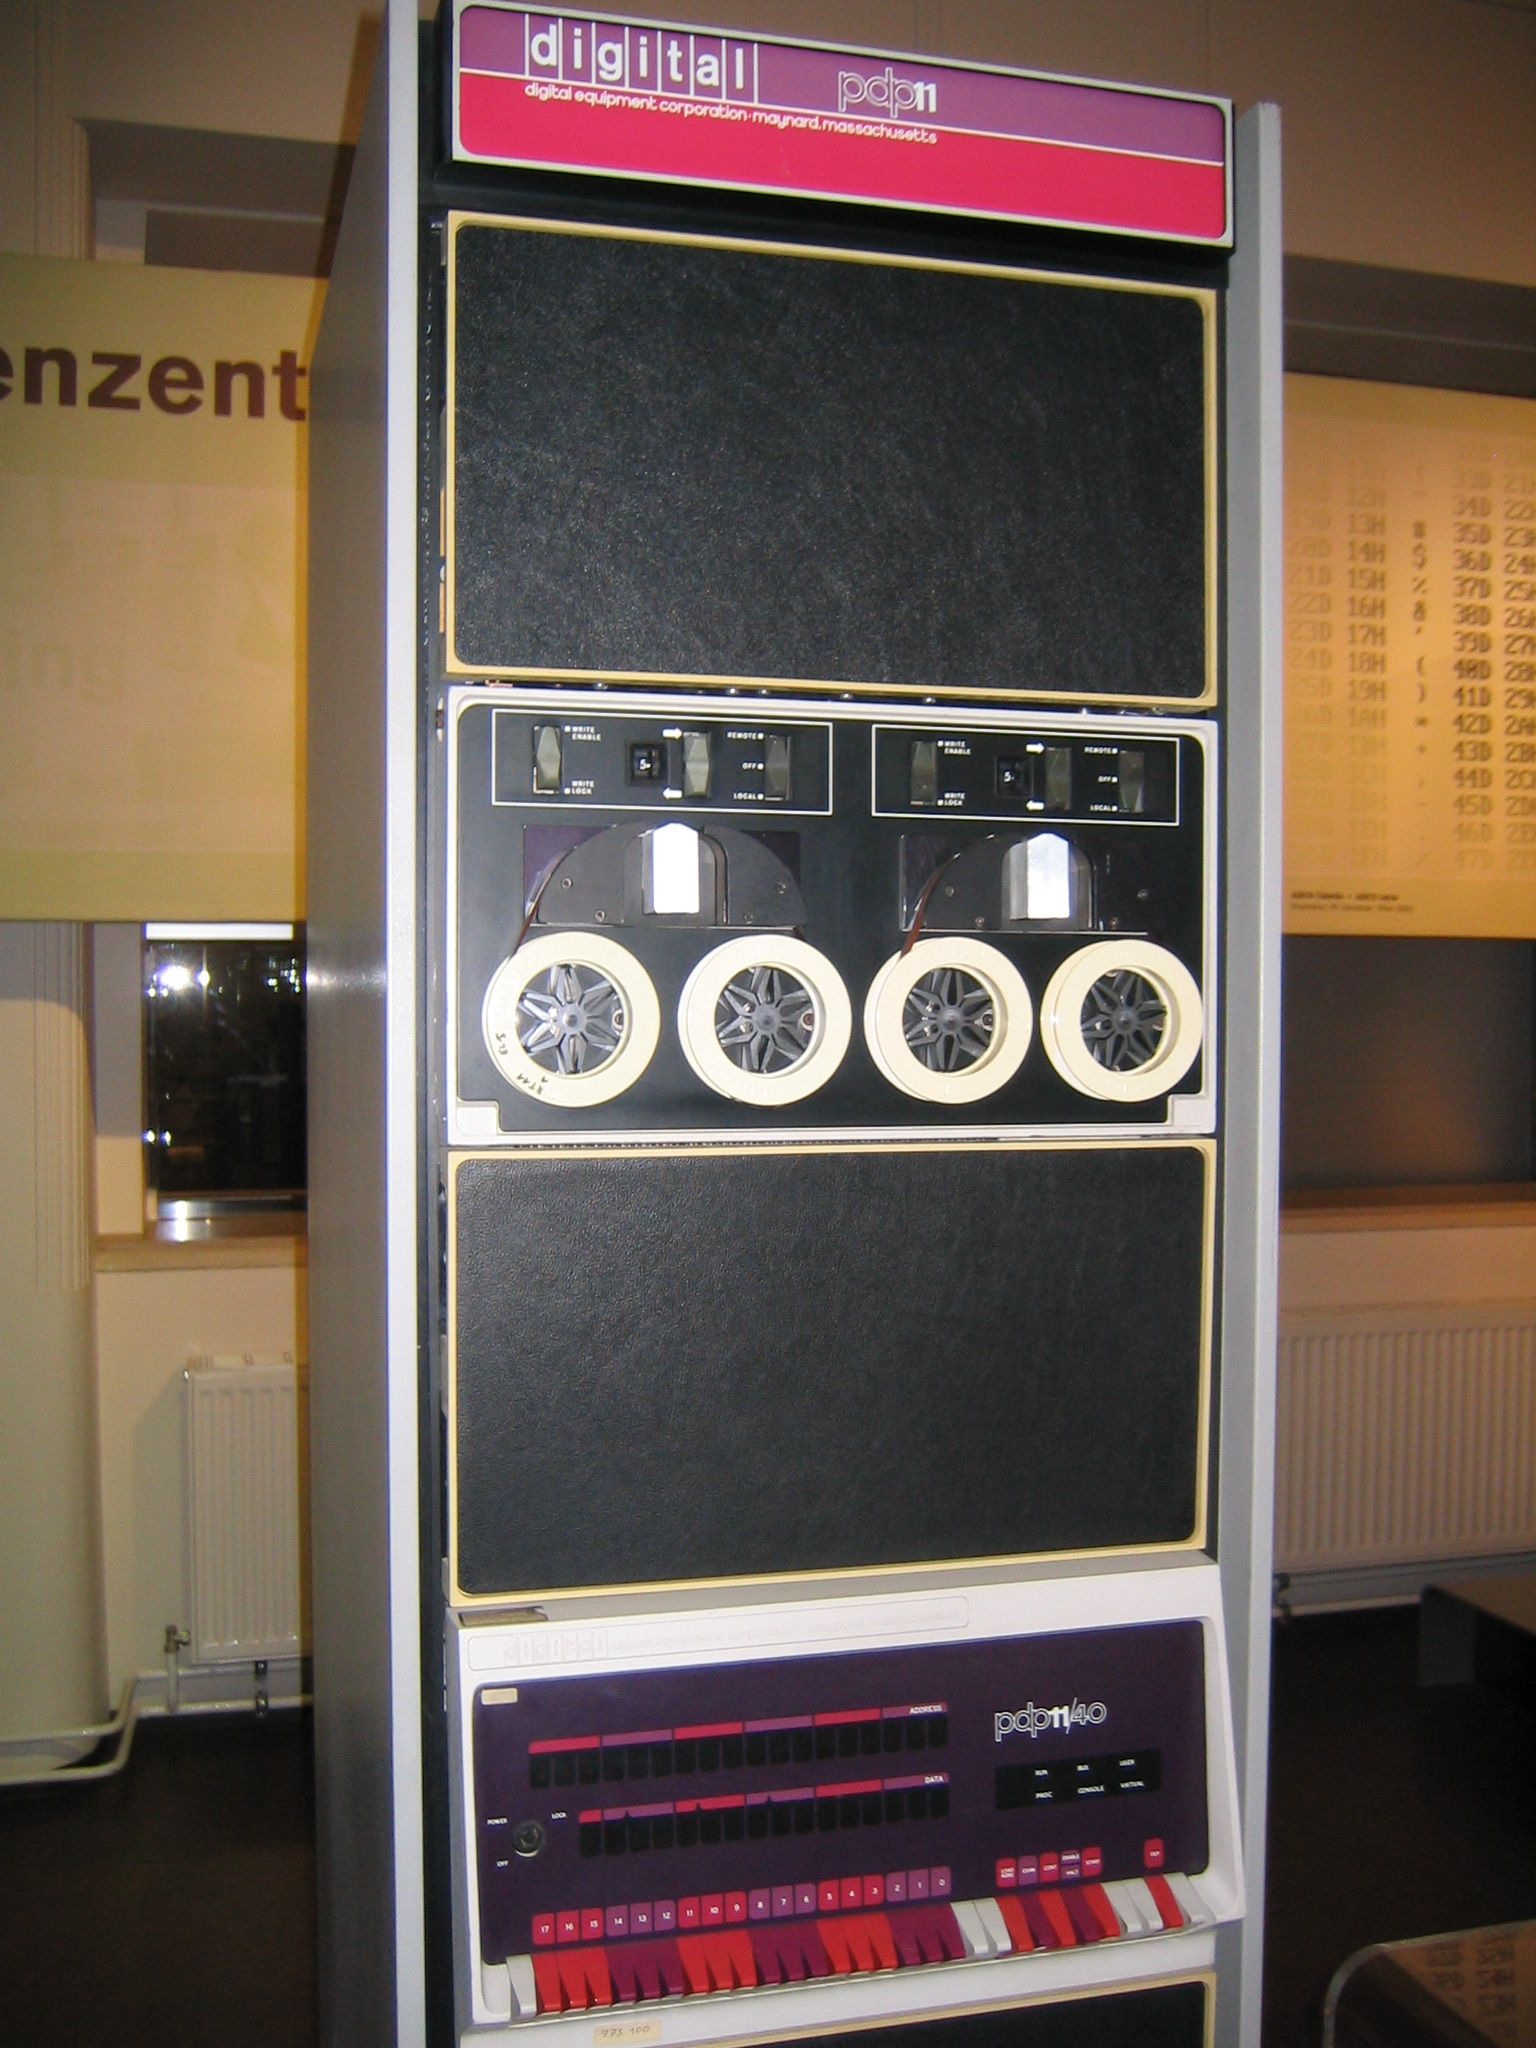
\includegraphics{pics/Pdp-11-40}}
\caption{\href{http://en.wikipedia.org/wiki/Image:Pdp-11-40.jpg}{PDP-11}}
\end{figure}
\end{columns}
\end{frame}

% %---------------------------------------------------------------------- SLIDE -
% \begin{frame}
% \frametitle{1960--1970: \href{http://en.wikipedia.org/wiki/PDP-11}{PDP-11}}
% \begin{figure}
% \center
% \scalebox{0.2}{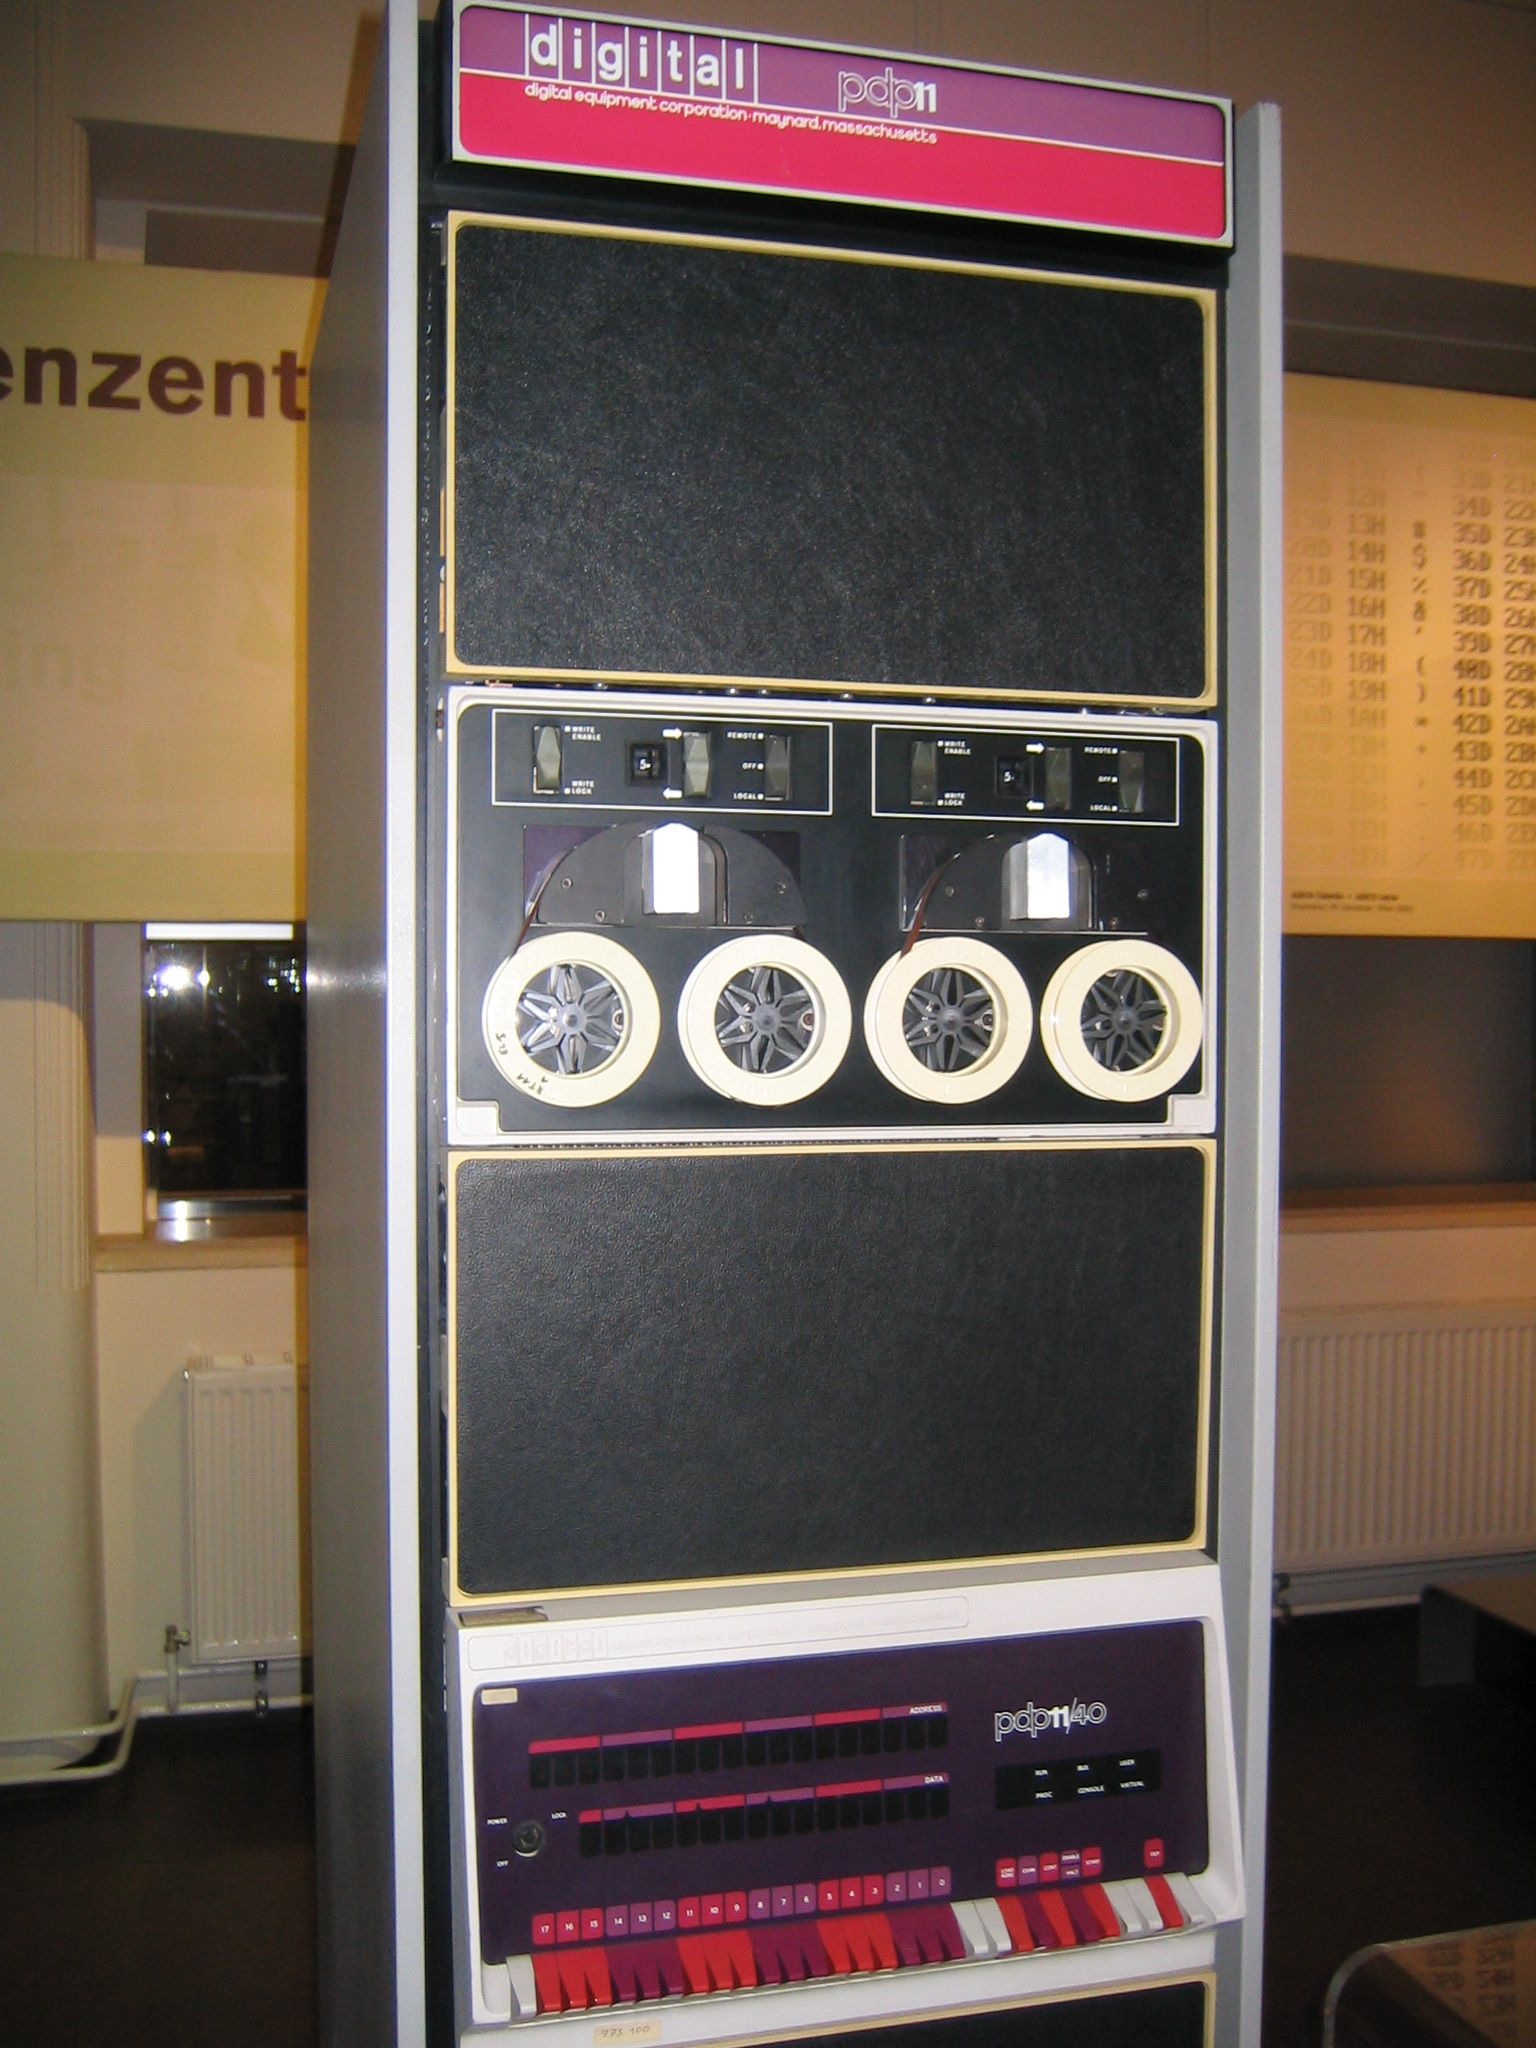
\includegraphics{pics/Pdp-11-40}}
% \caption{\href{http://en.wikipedia.org/wiki/Image:Pdp-11-40.jpg}{PDP-11}}
% \end{figure}
% \end{frame}

%-------------------------------------------------------------- SUBSUBSECTION -
\subsubsection{Многозадачност}

%---------------------------------------------------------------------- SLIDE -
\begin{frame}
\frametitle{1960--1970: Многозадачност}
\begin{itemize}
  \item В ранните операционни системи е типична еднозадачната обработка:
  \begin{itemize}
    \item в оперативната памет има само едно задание;
    \item когато програмата извършва входно/изходна операция, процесорът чака
    тази операция да завърши.
  \end{itemize}
\end{itemize}
\begin{figure}
\center
\scalebox{0.8}{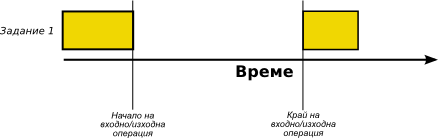
\includegraphics{pics/01-single-program-timeline}}
\caption{Еднозадачна обработка}
\end{figure}
\end{frame}

%---------------------------------------------------------------------- SLIDE -
\begin{frame}
\frametitle{1960--1970: Многозадачност}
\begin{columns}
\column{0.6\textwidth}
\begin{itemize}
  \item Процесорът е значително по-бърз от периферните устройства. Когато
  задачата е свързана с голям обем входно/изходни операции процесорът се
  използва много неефективно.
  \item С цел по-ефективно използване на процесора се преминава към многозадачна
  обработка:
  \begin{itemize}
    \item в оперативната памет едновременно се намират няколко задания;
    \item когато някое от заданията чака за изпълнение на входно/изходна
    операция, процесорът може да премине към обработване на друго задание.
  \end{itemize}    
\end{itemize}
\column{0.3\textwidth}
\begin{figure}
\center
\scalebox{0.5}{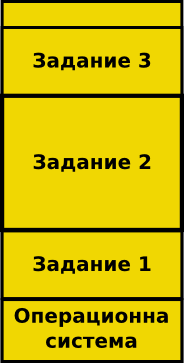
\includegraphics{pics/01-multiprogramming}}
\caption{Многозадачност}
\end{figure}
\end{columns}

\end{frame}


%---------------------------------------------------------------------- SLIDE -
\begin{frame}
\frametitle{1960--1970: Многозадачност}
\begin{figure}
\center
\scalebox{0.8}{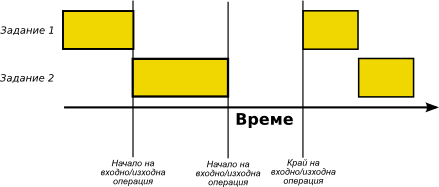
\includegraphics{pics/01-multiprogram-timeline}}
\caption{Многозадачна обработка}
\end{figure}
\end{frame}


%-------------------------------------------------------------- SUBSUBSECTION -
\subsubsection{Времеделене}

%---------------------------------------------------------------------- SLIDE -
\begin{frame}
\frametitle{1960--1970: Времеделене}
\begin{itemize}
  \item Организацията на работа при пакетната обработка е такава, че времето
  между подаването на заданието и получаването на резултатите е няколко часа.
  \item Желанието за по-кратко време на реакция води до възникването на идеята
  за времеделене - многозадачна работа, при която всеки потребител има терминал.
  \item Времето на процесора се разделя между всички потребители.
\end{itemize}
\end{frame}


%---------------------------------------------------------------------- SLIDE -
\begin{frame}
\frametitle{1960--1970: Времеделене}
\begin{table}
\begin{supertabular}{|p{0.15\textwidth}|p{0.35\textwidth}|p{0.35\textwidth}|}
\hline
\ & Пакетна обработка & Времеделене \\
\hline
Основна цел & 
Оптимизация на използването на процесора &
Минимизиране на времето за реакция \\
\hline
Въвеждане на команди &
Командите на езика за управление на заданията се  включват в заданието &
Командите се въвеждат от терминал\\
\hline
\end{supertabular}
\caption{Сравнение между пакетната обработка и времеделенето}
\end{table}
\end{frame}

%---------------------------------------------------------------------- SLIDE -
\begin{frame}
\frametitle{1960--1970: Времеделене --- \href{http://en.wikipedia.org/wiki/CTSS}{CTSS}}
\begin{itemize}
  \item Първата операционна система поддържаща времеделене е
  \href{http://en.wikipedia.org/wiki/Open_Source_history}{CTSS (Compatible 
  Time Sharing System)}
  \item Разработена в началото на 60-те (1963) в MIT
  \item Ръководител на проекта е
  \href{http://en.wikipedia.org/wiki/Fernando_J._Corbato}{Фернандо Корбато
  (Fernando J. Corbato)}  
  \item  \href{http://larch-www.lcs.mit.edu:8001/~corbato/sjcc62/}{Fernando J.
  Corbato, et al, AN EXPERIMENTAL TIME-SHARING SYSTEM, 1962} 
  \item Работи върху специално модифициран IBM 7094.
\end{itemize}
\end{frame}

%---------------------------------------------------------------------- SLIDE -
\begin{frame}
\frametitle{1960--1970: Времеделене --- \href{http://en.wikipedia.org/wiki/Multics}{MULTICS}}
\begin{itemize}
  \item Идеята за времеделене получава силно развитие благодарение на проекта MULTICS
  \item Планирането на проекта MULTICS започва през 1964.
  \item Проекта стартира със съвместното участие на MIT (Фернандо Корбато), GE
  и Bell Labs. 
  \item MULTICS има огромно въздействие върху развитието на операционните системи.
\end{itemize}
\end{frame}

%---------------------------------------------------------------------- SLIDE -
\begin{frame}
\frametitle{1960--1970: Времеделене --- \href{http://en.wikipedia.org/wiki/Multics}{MULTICS}}
\begin{figure}
\center
\scalebox{0.3}{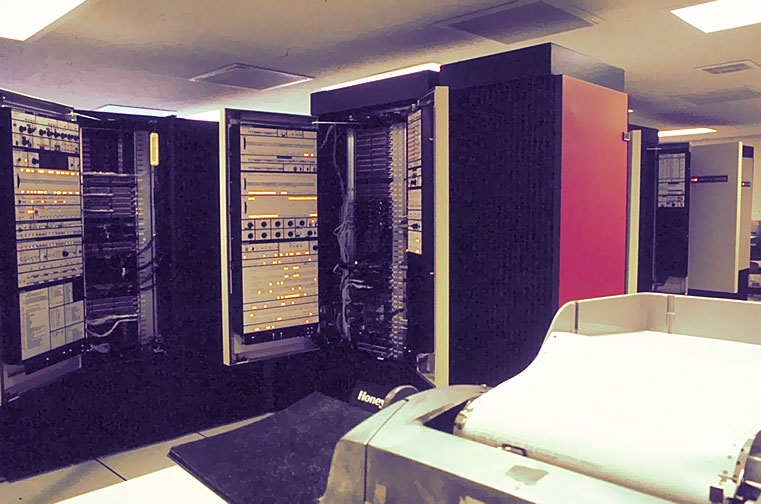
\includegraphics{pics/MULTICS-h6180-doors-open-big}}
\caption{\href{http://www.multicians.org/}{Multics върху Honeywell 6180}}
\end{figure}    
\end{frame}

%-------------------------------------------------------------- SUBSUBSECTION -
\subsubsection{UNIX}

%---------------------------------------------------------------------- SLIDE -
\begin{frame}
\frametitle{1960--1970: \href{http://en.wikipedia.org/wiki/Unix}{UNIX}}
\begin{itemize}
  \item В края на 60 те  започва работата по UNIX.
    \url{http://en.wikipedia.org/wiki/Unix}
	\url{http://www.bell-labs.com/history/unix}
    \url{http://www.levenez.com/unix}
%  \item Ранните операционни системи се разработват за всеки конкретен компютър.
  \item Екип от Bell Labs работи по проекта Multics от 1965. Идеята е била да се
  разработи удобна, интерактивна и икономична операционна система.
  \item През 1969 Bell Labs се оттеглят от работата по Multics, но част от екипът
  работил по проекта -- 
  \href{http://en.wikipedia.org/wiki/Ken_Thompson}{Кен Томпсън (Ken Thompson)},
  \href{http://en.wikipedia.org/wiki/Dennis_Ritchie}{Денис Ричи (Dennis Ritchie)},  
  \href{http://en.wikipedia.org/wiki/Doug_McIlroy}{Дъг Макилрой (Doug McIlroy)},
  \href{http://en.wikipedia.org/wiki/Joe_Ossanna}{Джо Осана (Joseph F. Ossanna)}
  -- продължава да се занимава с разработването на операционна система.
\end{itemize}
\end{frame}
    
%---------------------------------------------------------------------- SLIDE -
\begin{frame}
\frametitle{1960--1970: \href{http://en.wikipedia.org/wiki/Unix}{UNIX}}
\begin{itemize}
  \item Кен Томпсън в свободното си време разработва компютърната игра Space
  Travel. Първоначално играта е разработена за Multics, а след това е преписана
  на Fortran за GECOS и работи върху GE-635.
  \item Кен Томпсън и Денис Ричи пренаписват Space Travel за да работи върху
  PDP-7. За целта се използва кросасемблер, който работи върху GECOS, резултата
  се записва върху перфолента, която след това се зарежда за ипълнение върху
  PDP-7.
  \item За да облекчат работата по Space Travel, Томпсън и Ричи решават да
  имплементират върху PDP-7 част от вижданията си за операционните системи.
  \item През лятото на 1969 Томпсън последователно имплементира всички
  компоненти на UNIX.
  \item С това започва \href{http://www.levenez.com/unix}{дългата история} на
  UNIX. 
\end{itemize}
\end{frame}


%---------------------------------------------------------------------- SLIDE -
\begin{frame}
\frametitle{1960--1970: \href{http://en.wikipedia.org/wiki/Unix}{UNIX}}
\begin{figure}
\center
\scalebox{0.4}{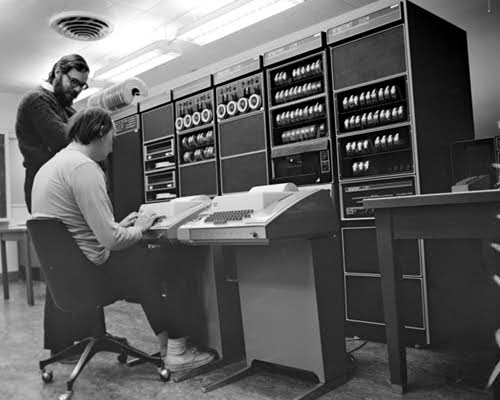
\includegraphics{pics/UNIX-PDP-11}}
\caption{\href{http://www.bell-labs.com/history/unix/firstport.html}{Денис Ричи
и Кен Томпсън}} 
\end{figure}
\end{frame}



%----------------------------------------------------------------- SUBSECTION -
\subsection{1970--1980}

%---------------------------------------------------------------------- SLIDE -
\begin{frame}
\frametitle{\href{http://en.wikipedia.org/wiki/History_of_computing_hardware_(1960s-present)}{
1970--1980}}
\begin{itemize}
  \item Развитие на интегрални схеми с голяма степен на интеграция -- LSI (Large
  Scale Integration) и VLSI (Very Large Scale Integration).
  \item Създаден е първият
  \href{http://en.wikipedia.org/wiki/Microprocessor}{микропроцесор}.
%   \item Three projects arguably delivered a complete microprocessor at about
%   the same time, namely Intel's 4004, Texas Instruments' TMS 1000, and Garrett
%   AiResearch's Central Air Data Computer
  \item Няколко проекта водят до създаването на микропроцесори, които се
  появяват по приблизително едно и също време:
  \begin{itemize}
    \item 1970: Garrett AiReserch - Central Air Data Computer (F14 Tomcat);
    \item 1971: Texas Instruments TMS 1000;
    \item 1971: Intel 4004.
  \end{itemize}
\end{itemize}
\end{frame}
  
  
%---------------------------------------------------------------------- SLIDE -
\begin{frame}
\frametitle{\href{http://en.wikipedia.org/wiki/History_of_computing_hardware_(1960s-present)}{
1970--1980}}
\begin{itemize}
  \item През 1972 Intel създава първият 8-битов микропроцесор - 8008.
  \item През 1974 се появява наследникът му -
  \href{http://en.wikipedia.org/wiki/Intel_8080}{8080}.
\begin{figure}
\center
\scalebox{1}{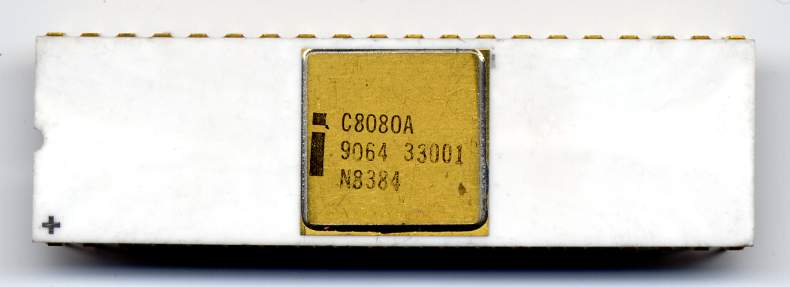
\includegraphics{pics/Intel_C8080A_9064_33001_N8384_top}}
\caption{\href{http://en.wikipedia.org/wiki/Image:Intel_C8080A_9064_33001_N8384_top.jpg}{Intel
8080}}
\end{figure}
\end{itemize}
\begin{itemize}            
  \item През 1974 се появява и конкурентът на 8080 - Motorola 6800.
  \item През 1978 Intel въвеждат 16-битовия процесор 8086, който ляга в
  основата на IBM PC.
\end{itemize}
\end{frame}

%---------------------------------------------------------------------- SLIDE -
\begin{frame}
\frametitle{\href{http://en.wikipedia.org/wiki/History_of_computing_hardware_(1960s-present)}{
1970--1980}}
\begin{itemize}
  \item През 70-те основно се разработват многопотребителски системи с
  времеделене.
  \item Продължава да се използва пакетна обработка на заданията.
  \item Под въздействие на развитието на микропроцесорите се появяват и първите
  \href{http://en.wikipedia.org/wiki/Microcomputer}{микрокомпютри (персонални компютри)}.
\end{itemize}
\end{frame}

%---------------------------------------------------------------------- SLIDE -
\begin{frame}
\frametitle{\href{http://en.wikipedia.org/wiki/History_of_computing_hardware_(1960s-present)}{
1970--1980}}
\begin{columns}
\column{0.5\textwidth}
\begin{figure}
\center
\scalebox{0.2}{\includegraphics{pics/MICROCOMPUTER-450px-Apple-II}}
\caption{\href{http://en.wikipedia.org/wiki/Apple_II_family}{Apple II}} 
\end{figure}
\column{0.5\textwidth}
\begin{figure}
\center
\scalebox{0.4}{\includegraphics{pics/MICROCOMPUTER-Trs80_2}}
\caption{\href{http://en.wikipedia.org/wiki/TRS_80}{TRS 80}} 
\end{figure}
\end{columns}
\end{frame}


%---------------------------------------------------------------------- SLIDE -
\begin{frame}
\frametitle{
1970--1980: \href{http://en.wikipedia.org/wiki/Tcp/ip}{TCP/IP}}
\begin{itemize}
  \item В началото на 70-те DARPA (Defense Advanced Research Projects Agency)
    разработва TCP/IP.
  \item Първоначално реализации на TCP/IP се разработват от BBN Technologies,
  Stanford University,  и University College London.
  \item TCP/IP се превръща в стандартен комуникационен протокол.
\end{itemize}
\end{frame}


%----------------------------------------------------------------- SUBSECTION -
\subsection{1980--1990}

%---------------------------------------------------------------------- SLIDE -
\begin{frame}
\frametitle{\href{http://en.wikipedia.org/wiki/History_of_computing_hardware_(1960s-present)}{
1980--1990}}
\begin{itemize}
  \item В началото на 80-те IBM разработва
  \href{http://en.wikipedia.org/wiki/IBM_PC}{IBM PC}. Това поставя началото на 
  ерата на персоналните компютри. 
\end{itemize}
\begin{figure}
\center
\scalebox{0.2}{\includegraphics{pics/IBM_PC_5150}}
\caption{\href{http://en.wikipedia.org/wiki/IBM_PC}{IBM PC, модел 5150}} 
\end{figure}

\end{frame}

%---------------------------------------------------------------------- SLIDE -
\begin{frame}
\frametitle{\href{http://en.wikipedia.org/wiki/History_of_computing_hardware_(1960s-present)}{
1980--1990}}
\begin{itemize}
   \item Персоналните компютри рязко променят начина, по който се използват компютри.
   \item Компютрите стават достъпни и се разпространяват навсякъде, където има
   нужда от тях.
   \item Персоналните компютри се доказват като лесни за употреба.
   \item С развитието на хардуера използването на
   \href{http://en.wikipedia.org/wiki/History_of_the_graphical_user_interface}{графичен интерфейс} се превръща 
    в стандарт.
   \item Пренасянето на информация между компютрите посредством
   \href{http://en.wikipedia.org/wiki/Computer_networking}{компютърни мрежи} 
   става достатъчно евтино и практично.
   \item Широко разпространение получава клиент/сървър модела за разработване на
    приложения.
   \begin{itemize}
     \item клиентите изпращат заявки за различни услуги към сървъра;
     \item сървъра обработва заявките и връща отговор.
   \end{itemize}
%    \item 
%     Software engineering field continued to evolve
%         Major thrust by the United States government aimed at tighter control of Department of Defense software projects
%             Realizing code reusability
%             Greater degree of abstraction in programming languages
%             Multiple threads of instructions that could execute independently
%   \item 
\end{itemize}
\end{frame}
  

%----------------------------------------------------------------- SUBSECTION -
\subsection{1990--2000}

%---------------------------------------------------------------------- SLIDE -
\begin{frame}
\frametitle{\href{http://en.wikipedia.org/wiki/History_of_computing_hardware_(1960s-present)}{
1990--2000}}
\begin{itemize}
  \item Производителността на хардуера нараства експоненциално.
  \item Напредъка в технологиите намалява цените на изчислителната мощност и
  запаметяващите устройства.
  \item Големите машини стават рядкост.
\end{itemize}
\end{frame}


%---------------------------------------------------------------------- SLIDE -
\begin{frame}
\frametitle{\href{http://en.wikipedia.org/wiki/History_of_computing_hardware_(1960s-present)}{
1990--2000}}
\begin{figure}
\center
\scalebox{0.35}{\includegraphics{pics/Moore_Law}}
\caption{\href{http://en.wikipedia.org/wiki/Image:Moore_Law_diagram_(2004).png}{Закон на Мур}} 
\end{figure}

\end{frame}


%---------------------------------------------------------------------- SLIDE -
\begin{frame}
\frametitle{\href{http://en.wikipedia.org/wiki/History_of_computing_hardware_(1960s-present)}{
1990--2000}}
\begin{itemize}
  \item Ускорява се преходът към разпределени системи.
  \item Поддръжката на мрежови функции от операционните системи става стандарт.
  \item Операционната система Windows на Microsoft става доминираща.
\end{itemize}
\end{frame}


%---------------------------------------------------------------------- SLIDE -
\begin{frame}
\frametitle{\href{http://en.wikipedia.org/wiki/History_of_computing_hardware_(1960s-present)}{
1990--2000}}
\begin{itemize}
  \item Обектната технология на програмиране става доминираща.
  \item Разработват се много обектно-ориентирани езици за програмиране --
  Smalltalk, C++, Java и т.н.
  \item Обектните технологии навлизат и в разработването на операционни системи
  -- обектно ориентирани операционни системи (OOOS).
  \item Концепциите на обектно-ориентираното програмиране се използват за
  разработване на модулни операционни системи.
  \item По-голямата част от софтуера се продава (разпространява) като изпълним
  код. 
\end{itemize}
\end{frame}


%---------------------------------------------------------------------- SLIDE -
\begin{frame}
\frametitle{\href{http://en.wikipedia.org/wiki/History_of_computing_hardware_(1960s-present)}{
1990--2000}}
\begin{itemize}
  \item  През 1983г. 
  \href{http://en.wikipedia.org/wiki/Richard_Stallman}{Ричард Столман
  (Richard Stallman)}  стартира проекта \href{http://en.wikipedia.org/wiki/GNU}{GNU}.
\item През 90-те години
\href{http://en.wikipedia.org/wiki/Free_software_movement}{свободният
софтуер (free software)} и
\href{http://en.wikipedia.org/wiki/Open_Source_history}{софтуерът с
отворен код (open source software)} започват да придобиват популярност. 
\item Софтуерът с отворен код се разпространява заедно със сорс кода на
приложението. 
\item Това позволява на всеки да изучава и променя софтура за да удовлетвори
някакви специфични нужди.
\item През февруари 1998 е основана
\href{http://en.wikipedia.org/wiki/Open_Source_history}{Open Source Initiative (OSI)}.
\end{itemize}
\end{frame}


\end{document}